%% FEUP THESIS STYLE for LaTeX2e
%% how to use feupteses (portuguese version)
%%
%% FEUP, JCL & JCF, 31 Jul 2012
%%
%% PLEASE send improvements to jlopes at fe.up.pt and to jcf at fe.up.pt
%%
%%========================================
%% Commands: pdflatex tese
%%           bibtex tese
%%           makeindex tese (only if creating an index) 
%%           pdflatex tese
%% Alternative:
%%          latexmk -pdf tese.tex
%%========================================

\documentclass[11pt,a4paper,openright]{report}

%% For iso-8859-1 (latin1), comment next line and uncomment the second line
\usepackage[utf8]{inputenc}
%\usepackage[latin1]{inputenc}

%% Portuguese version

%% MIEIC options
\usepackage[portugues,mieic]{feupteses}
%\usepackage[portugues,mieic,juri]{feupteses}
%\usepackage[portugues,mieic,final]{feupteses}
%\usepackage[portugues,mieic,final,onpaper]{feupteses}

%% For other degrees
\usepackage[portugues]{feupteses} % you must define the degree bellow

%% Options: 
%% - portugues: titles, etc in portuguese
%% - onpaper: links are not shown (for paper versions)
%% - backrefs: include back references from bibliography to citation place

%% Uncomment to create an index (at the end of the document)
%\makeindex

%% Path to the figures directory
%% TIP: use folder ``figures'' to keep all your figures
\graphicspath{{figures/}}

%%----------------------------------------
%% TIP: if you want to define more macros, use an external file to keep them
%some macro definitions

% format
\newcommand{\class}[1]{{\normalfont\slshape #1\/}}

% entities
\newcommand{\Feup}{Faculdade de Engenharia da Universidade do Porto}

\newcommand{\svg}{\class{SVG}}
\newcommand{\scada}{\class{SCADA}}
\newcommand{\scadadms}{\class{SCADA/DMS}}

%%----------------------------------------

%%========================================
%% Start of document
%%========================================
\begin{document}

%%----------------------------------------
%% Information about the work
%%----------------------------------------
\title{Visage}
\author{Pedro Tiago Pontes}

%% Comment next line if not necessary for degree name
\degree{Mestrado Integrado em Engenharia Informática e Computação}

%% Uncomment next line for date of submission
%\thesisdate{31 de Julho de 2013}

%% Comment next line for copyright text if not used
\copyrightnotice{Pedro Tiago Pontes, 2013}

\supervisor{Orientador}{Cristina Ribeiro}

%% Uncomment next line if necessary
\supervisor{Co-orientador}{Filipe Coelho}

%% Uncomment committee stuff in the final version if used
%\committeetext{Aprovado em provas públicas pelo Júri:}
%\committeemember{Presidente}{Nome do presidente do júri}
%\committeemember{Arguente}{Nome do arguente do júri}
%\committeemember{Vogal}{Nome do vogal do júri}
%\signature

%% Specify cover logo (in folder ``figures'')
\logo{uporto-feup.pdf}
 
%% Uncomment next line for additional text below the author's name (front page)
%\additionalfronttext{Preparação da Dissertação}

%%----------------------------------------
%% Preliminary materials
%%----------------------------------------

% remove unnecessary \include{} commands
\begin{Prolog}
%%  \chapter*{Resumo}
%\addcontentsline{toc}{chapter}{Resumo}
O reconhecimento facial é efetuado de forma rotineira e quase sem esforço por parte das pessoas no seu dia-a-dia. No entanto, a construção de sistemas automáticos de reconhecimento facial é uma tarefa complexa que engloba um conjunto de sub-problemas específicos, nomeadamente a deteção e segmentação das faces presentes na imagem, a sua normalização e a extração das características distintivas das faces, para que, por fim, seja efetuado o reconhecimento da identidade das pessoas representadas. À resolução com sucesso deste conjunto de sub-problemas, colocam-se também um conjunto de desafios dos quais se destacam a variação ao nível da pose, iluminação e expressão das pessoas representadas.

Os desafios inerentes ao processo de reconhecimento, assim como a vasta gama de aplicações onde a identificação de indivíduos é necessária, como por exemplo o controlo de acesso a informação, a segurança, a aplicação da lei, o entretenimento e a gestão de conteúdos multimédia, despoletou a atenção de inúmeros investigadores ao longo dos últimos 40 anos. Como consequência, verificou-se uma evolução notável ao nível da eficácia dos sistemas desenvolvidos, considerando-se mesmo que o problema de reconhecimento facial em cenários cooperativos e com condições de captura de imagens controladas se encontra praticamente resolvido. Por outro lado, em cenários não cooperativos e onde se regista uma variação não controlada da captura das imagens, esta é ainda uma área de investigação em aberto. 

Os filtros de abstração constituem uma forma moderna de simplificação do conteúdo visual, permitindo remover informação redundante e dar destaque à mensagem visual a transmitir.

O projeto Visage visou o desenvolvimento de um sistema de reconhecimento facial de personalidades, baseado em código aberto, onde seja utilizada a abstração de imagens juntamente com um conjunto de outras tarefas de pré-processamento sobre as imagens a reconhecer. Com o sistema desenvolvido foi analisado o impacto dos filtros de abstração e das restantes tarefas de pré-processamento utilizadas no processo de reconhecimento. A avaliação de desempenho foi efetuada com recurso à biblioteca de imagens \textit{Labelled Faces in the Wild}, sobre duas perspetivas, \textit{Closed-set identification} e \textit{Image Retrieval}, e utilizando nove cadeias de pré-processamento de imagens distintas. Foram reportados para os resultados obtidos nos algoritmos \textit{Eigenfaces, Fisherfaces e LBPH}.

Os resultados demonstram que a aplicação de filtros de abstração no processo de reconhecimento resulta num compromisso entre a diminuição dos requisitos de armazenamento das imagens e uma ligeira diminuição da eficácia da identificação. Ao nível das restantes tarefas de pré-processamento, a deteção e segmentação das faces presentes nas imagens revelou ser a fase de pré-processamento com maior importância para a obtenção de resultados positivos. Por último, dos três algoritmos analisados, o algoritmo \textit{LBPH} revelou ter o melhor desempenho na maioria dos conjuntos analisados.

\chapter*{Abstract}
%\addcontentsline{toc}{chapter}{Abstract}
Face recognition is performed in a routine and effortless way by people in their daily life. However, building automated face recognition systems is a complex task that involves a set of specific sub-problems, namely face detection and segmentation, normalization of the extracted face and the extraction of the distinguishing features of the face, so that the recognition of the person present in a picture can be performed. In order to solve each of sub-problems with success, a set of challenges must be overcome, from which variation in pose, illumination and facial expression can be highlighted.

The challenges associated with the recognition process, as well as the wide range of areas where the identification of people is required, such as information access control, security, law enforcement, entertainment and multimedia content management, raised the attention of numerous researchers in the past 40 years. Consequently, a remarkable evolution was noticed in terms of system's performance. In cooperative scenarios with controlled image capturing conditions, it is considered that the problem of face recognition is almost solved. On the other hand,  in non-cooperative scenarios this is still an open research area.

Abstraction filters are a modern way to simplify visual content, allowing the removal of useless detail and the use of abstraction for effective communication.

The Visage project proposes the development of a face recognition system for public figures, based in open source libraries, where image abstraction along with some other pre-processing techniques are used in the process of recognition. The system has been used to analyse the impact of abstraction filters and the other pre-processing steps in face recognition. The performance was evaluated in Closed-set Identification and Image Retrieval perspectives, using the Labelled Faces in the Wild image library, with nine different pre-processing chains. Results were reported for Eigenfaces, Fisherfaces and Local Binary Patterns Histograms algorithms.

Results show that using abstraction filters in the process of automated face recognition results in a trade-off between reducing the images' storage requirements and a small decrease in the effectiveness of identification. Regarding the other pre-processing techniques, face detection and segmentation have shown the bigger positive impact on the results. Finally, three algorithms used in the analysis, Local Binary Patterns Histogram obtained the best performance in most of the analysed sets.  % the abstract
%%  \chapter*{Agradecimentos}
%\addcontentsline{toc}{chapter}{Agradecimentos}
A elaboração da presente dissertação constitui um marco fundamental da minha formação académica e pessoal. Gostaria de agradecer a todos os que contribuíram para que a conclusão desta etapa com sucesso e prazer.

\vspace{2mm}
Em primeiro lugar, gostaria de agradecer à Professora Maria Cristina Ribeiro e ao Engenheiro Filipe Coelho, pela supervisão, dedicação e apoio prestado na realização desta dissertação.

\vspace{2mm}
Um especial agradecimento aos meus pais e aos meus irmãos, pelo apoio constante, pela confiança, pela educação e valores que me transmitiram e por me proporcionarem todas as condições necessárias para ter sucesso.

\vspace{2mm}
À Maria João pelo apoio, carinho e confiança incondicionais.

\vspace{2mm}
Aos restantes amigos, porque sem vocês a conclusão desta etapa não teria o mesmo sentido.

\vspace{10mm}
Este trabalho foi parcialmente financiando pelo Sapo Labs da Universidade de Porto.

\flushleft{Pedro Tiago Carvalho da Silva Pontes}
  % the acknowledgments
%%  \cleardoublepage
\thispagestyle{plain}

\vspace*{8cm}

\begin{flushright}
   \textsl{``You should be glad that bridge fell down. \\
           I was planning to build thirteen more to that same design''} \\
\vspace*{1.5cm}
           Isambard Kingdom Brunel
\end{flushright}
    % initial quotation if desired
  \cleardoublepage
  \pdfbookmark[0]{Conteúdo}{contents}
  \tableofcontents
  \cleardoublepage
  \pdfbookmark[0]{Lista de Figuras}{figures}
  \listoffigures
  \cleardoublepage
  \pdfbookmark[0]{Lista de Tabelas}{tables}
  \listoftables
  \chapter*{Abreviaturas e Símbolos}
%\addcontentsline{toc}{chapter}{Abbreviations}
\chaptermark{ABREVIATURAS E SÍMBOLOS}

\begin{flushleft}
\begin{tabular}{l p{0.8\linewidth}}
API		& \textit{Application Programming Interface} (Interface de Programação de Aplicações) \\
CPU		& \textit{Central Processing Unit} (Unidade central de processamento)\\
FAR     & \textit{False Accept Rate} \\
FRR		& \textit{False Reject Rate} \\
LBP 	& \textit{Local Binary Patterns}\\
LBPH	& \textit{Local Binary Patterns Histograms}\\
LFW		& \textit{Labeled Faces in the Wild}\\
FERET   & \textit{Face Recognition Technology}\\
FRVT    & \textit{Facial Recognition Vendor Test}\\
GPU		& \textit{Graphics Processing Unit} (Unidade de Processamento Gráfico)\\
HCInt	& \textit{High Computational Intesity test}\\
LDA		& \textit{Linear Discriminant Analysis}\\
MBE		& \textit{Multiple Biometric Evaluation}\\
MCF		& \textit{Mean Curvature Flow}\\
MCInt	& \textit{Medium Computational Intensity test}\\
NIST	& \textit{National Institute of Standards and Technology} \\
OpenCV	& \textit{Open Source Computer Vision Library} \\
PCA		& \textit{Principal Component Analysis}\\
RAPID	& Reconhecimento Automático de Passageiros Identificados Documentalmente \\
ROC		& receiver operating characteristic\\
\end{tabular}
\end{flushleft}

  % the list of abbreviations used
\end{Prolog}

%%----------------------------------------
%% Body
%%----------------------------------------

\StartBody

%% TIP: use a separate file for each chapter
\chapter{Introdução} \label{chap:intro}

A sociedade atual caracteriza-se pelo constante fluxo de informação a que os seus indivíduos estão expostos, assistindo-se a um crescimento acelerado na produção de conteúdos multimédia, principalmente tendo em conta os meios de transmissão de informação digital \citep{IntelCorporation}. O aparecimento de novas formas de comunicação, como por exemplo as redes sociais, e uso de um maior leque de dispositivos para a produção de conteúdos como por exemplo \textit{smarphones} e \textit{tablets}, intensificou ainda mais este crescimento, contribuindo também para o surgimento de conteúdos cada vez mais personalizados e variados. Neste contexto, torna-se importante o desenvolvimento de novas metodologias que possibilitem a categorização, organização e posterior pesquisa por porte dos utilizadores destes conteúdos, representando o reconhecimento facial automático em imagens um papel importante a esse nível.

O reconhecimento facial é um componente importante da capacidade de perceção humana, sendo efetuado de uma forma rotineira e quase sem esforço por parte dos seres humanos. Contudo, a construção de sistemas computacionais capazes de efetuar este tipo de reconhecimento de uma forma semelhante aos humanos é ainda uma área de investigação em aberto \citep{Li2011}. Este é um problema de tal forma desafiante e interessante que tem despertado a atenção de investigadores das mais diversas áreas, ao longo dos últimos 40 anos, tais como: psicologia, reconhecimento de padrões, redes neuronais, visão por computador e computação gráfica \citep{Zhao2003}.

Por outro lado, a abstração de imagens dota os artistas de novas ferramentas de transmissão de informação, tendo como objetivo, melhorar eficácia da comunicação visual. Os filtros de abstração permitem remover informação não essencial de uma imagem, dando apenas destaque à mensagem a transmitir. 

No âmbito desta dissertação, é levantada a seguinte hipótese: O uso de abstração em imagens que vão ser posteriormente alvo de reconhecimento facial, pode melhorar o processo de reconhecimento. Este impacto deverá ser analisado do ponto de vista da eficácia do reconhecimento, mas também ao nível das necessidades de processamento e armazenamento das coleções de dados a reconhecer.

\section{Motivação} \label{sec:motivation}
O reconhecimento facial automático em imagens é uma área de investigação em aberto, principalmente quando considerados ambientes onde onde as condições de captura de imagens não são controladas, uma situação muito comum na grande maioria das bibliotecas de imagens existentes. Nessas situações, as grandes variações existentes ao nível da iluminação, pose e expressão dos indivíduos propõem grandes desafios à tarefa de reconhecimento facial automático para os quais existe ainda a necessidade de evoluir as soluções existentes.

A pesquisa ao nível do reconhecimento facial é motivada não só pelos desafios inerentes ao processo de reconhecimento facial, mas também, pelas inúmeras aplicações onde a identificação de indivíduos é necessária \citep{Li2011}. A esse nível, a evolução tecnológica registada nos últimos vinte anos culminou com o surgimento de uma panóplia de dispositivos e áreas onde se verifica um aumento do interesse na aplicação desta tecnologia, desde a mais tradicional segurança e controlo de informação, a áreas como o entretenimento ou a gestão de conteúdos multimédia e bases de dados. Ao nível dos dispositivos, o surgimento de novas plataformas, e o aumento da capacidade de computação das já existentes, torna possível a aplicação destes sistemas, não só em máquinas dedicadas para o efeito, mas  também em computadores pessoais ou mesmo em dispositivos móveis como \textit{smartphones} ou \textit{tablets}.

Por outro lado, o elevado valor comercial associado aos sistemas de reconhecimento facial existentes, tem como  consequência a existência de um número reduzido de soluções abertas, fazendo com que os resultados eventualmente obtidos no âmbito desta dissertação possam ter uma boa visibilidade.

Finalmente, a aplicação de filtros de abstração de imagens para a ilustração automática de texto demonstrou melhorias ao  nível da informação retornada, assim como, na redução significativa das necessidades de processamento e armazenamento necessárias \citep{Coelho:2012:IAC:2260641.2260676}, tornando-se assim pertinente o estudo do impacto dos filtros de abstração no processo de reconhecimento facial no âmbito desta dissertação.

\section{Objetivos} \label{sec:objetivosintro}
O principal objetivo deste projeto visa o estudo do impacto de filtros de abstração visual de informação no processo de reconhecimento facial automático em imagens. Para isso, destacam-se o seguinte conjunto de objetivos parciais:

\begin{enumerate}
\item Desenvolvimento de um sistema de reconhecimento facial de personalidades;
\item Integração da abstração de imagens no sistema desenvolvido;
\item Avaliação dos resultados da abstração de imagens no processo de reconhecimento facial;
\end{enumerate}

O sistema desenvolvido deverá ser capaz de detetar as faces presentes numa imagem e apresentar uma lista de possíveis entidades nela contidas.

Da avaliação efetuada, para além da publicação desta dissertação, espera-se ainda a publicação de um artigo científico onde sejam descritos os resultados obtidos.

\section{Estrutura do Relatório} \label{sec:struct}
Este relatório encontra-se dividido em quatro capítulos. Após uma breve introdução, é efetuada, no segundo capítulo, uma revisão do problema de reconhecimento facial automático em imagens, analisando os desafios existentes, as suas diversas áreas de aplicação e as estratégias adotadas para os sistemas atualmente existentes. No terceiro capítulo deste relatório, é abordado o tema da abstração de imagens, ilustrando as soluções existentes, assim como o trabalho relacionado com esta dissertação efetuado com  recurso à abstração de imagens. Por último, no quarto capítulo, é apresentada a perspetiva de solução a desenvolver, nomeadamente os detalhes da sua implementação, a forma como temos em vista analisar o desempenho do sistema e o plano de trabalho previsto.
\chapter{Reconhecimento Facial em Imagens} \label{chap:reco}

A capacidade de distinguir indivíduos através das suas características faciais é inata aos seres humanos, efetuada uma forma natural e quase sem esforço. A forma como efetuamos esse reconhecimento, é no entanto um problema complexo, que atrai a atenção de investigadores das mais diversas áreas, sendo da psicologia e na década de 50 \citep{BRUNERJEROMES.TAGIURI1954}, o mais antigo estudo efetuado sobre o tema. Associado a este problema, o reconhecimento facial automático, ou seja, o reconhecimento facial efetuado de uma forma automática com o auxílio de máquinas tais como computadores, tem de igual forma recebido muita atenção por tarte da comunidade científica, sendo que o primeiro sistema de reconhecimento facial automático de que há registo, foi desenvolvido da década de 70 por Takeo Kanade \citep{Kanade1973}. Ao longo dos anos, investigadores das mais diversas áreas, tais como  psicologia, reconhecimento de padrões, neurologia, visão por computador ou computação gráfica, efetuaram estudos em vários aspetos do reconhecimento facial efetuado por computadores e máquinas.

Ao nível do reconhecimento facial automático, após o trabalho de Kanade, e outros realizados por alguns dos seus pares na década de 70, verificou-se um abrandamento na investigação científica efetuada na área até meados dos anos 90, onde o trabalho realizado por Turk e Pentland \citep{Turk1991} trouxe um novo impulso ao desenvolvimento de sistemas e metodologias de reconhecimento facial automático. Neste estudo, Turk e Pentland apresentaram uma nova forma abordagem ao reconhecimento facial designada de \textit{Eingenfaces}. Um outro marco no desenvolvimento nas metodologias de reconhecimento facial, foi o surgimento do método \textit{Fisherfaces} \citep{Belhumeur1997, Zhao1998}, o qual apresenta uma maior insensibilidade em relação à variação da iluminação e expressões faciais presentes nas imagens.

Ao longo da década de 90 a investigação científica na área do reconhecimento facial automático intensificou-se, tendência que ainda se verifica atualmente, tal como pode ser verificado pelo surgimento de várias conferências, das quais são exemplo, desde as mais antigas
\textit{International Conference on Automatic Face and Gesture Recognition (AFGR)} (1995) e \textit{International Conference on Audio- and Video-Based Authentication (AVBPA)} (1997), até à recentemente realizada \textit{5th International Conference on Biometrics (ICBS)} (2012).

Paralelamente, o surgimento de programas como o Face Recognition Technology (FERET) (1993-1998), levado a cabo pelo \textit{National Institute of Standards and Technology (NIST)} dos E.U.A, com o objetivo de financiar a investigação na área e estabelecer padrões para a avaliação das diversas metodologias de reconhecimento facial criadas, assim como impulsionar a criação de uma base de dados de faces de grande dimensões para o teste dos sistemas criados, permitiu uma evolução significativa na área \citep{Phillips1998, Phillips2000}.

No final da década de 90, surgiram as primeiras aplicações comerciais de reconhecimento facial automático, tal como pode ser comprovado  pela participação de 5 soluções comerciais na primeira edição dos \textit{Facial Recognition Vendor Test (FRVT)}, no ano 2000 \citep{BlackburnDuaneM.;BoneMike;Phillips2001}. Nesta avaliação, as soluções eram testadas nas componentes de usabilidade e performance do reconhecimento efetuado, de modo fornecer uma avaliação objetiva e independente dos sistemas de reconhecimento facial presentes no mercado. Estas avaliações foram repetidas nos anos de 2002, 2006, 2010 e 2012.

Neste capítulo, em primeiro lugar, é efetuada uma definição do problema de reconhecimento facial automático, assim como dos sub-problemas que o compõem e dos desafios existentes para a sua resolução. De seguida, são apresentadas as diversas áreas de aplicação do reconhecimento facial automático. Em terceiro lugar, é apresentada uma revisão das estratégias utilizadas para a implementação de sistema de reconhecimento facial automático, assim como dos diversos sistemas existentes. Por último, é efetuada uma revisão das avaliações efetuadas no âmbito dos programas FERET e FRVT, aos sistemas de reconhecimento facial existentes.

\section{Definição do Problema} \label{sec:problema}
De uma forma geral, o problema de reconhecimento facial pode ser formulado da seguinte forma: dada uma imagem (prova), pretende-se identificar ou verificar a presença de uma ou mais pessoas na prova, comparando-a com uma base de dados de faces previamente guardada (galeria) \citep{Yang2002, Zhao2003}. Este problema, pode ainda ser dividido em dois sub-problemas específicos: verificação de faces (ou autenticação) e identificação de faces \citep{Li2011}:

\begin{description}
\item[Verificação] Uma prova é apresentada ao sistema, assim como a respetiva identidade da pessoa presente na imagem. Cabe ao sistema verificar se existe uma correspondência entre a pessoa representada na imagem e a identidade fornecida. Assim, é efetuada uma comparação 1:1, que responde à pergunta: "Esta pessoa é quem realmente afirma ser?".

\item[Identificação] Uma prova é apresentada ao sistema, e pretende-se que este devolva a identidade da pessoa presente na imagem, assim como o nível de confiança associado à correspondência efetuada entre a imagem e a identidade devolvida. A identificação de faces pode ainda ser dividida em dois sub-problemas: 

No primeiro problema designado \textit{watch list} ou \textit{open-set identification}\citep{Chellappa2010}, não é garantido que o sistema conheça a pessoa a ser identificada, pelo que em primeiro lugar é necessário identificar se a pessoa existe na galeria e, caso exista, determinar a identidade da pessoa. Este sub-problema responde às perguntas: "Esta pessoa está presente na galeria? Se sim, de quem é esta face?". 

O segundo caso, é aquele que é geralmente avaliado em sistemas de reconhecimento facial, onde é garantido que a pessoa é conhecida pelo sistema, respondendo-se apenas à pergunta: "De quem é esta face?". Nesta situação, designada de \textit{closed-set identification}, podem ainda ser pedidas todas as correspondências efetuadas com um nível de confiança superior a um valor pré-definido. 
Em qualquer um dos subproblemas de identificação, é efetuada uma comparação 1:N.
\end{description}

Os sistemas de reconhecimento facial podem ainda ser divididos genericamente em dois grupos, tendo em conta a fonte de onde são extraídas as faces a analisar. O primeiro grupo baseia-se no uso de imagens estáticas, como por exemplo fotografias de personalidades ou mesmo em retratos de faces humanas criadas por ilustradores. O segundo, tem por base o uso de vídeos, dos quais são extraídas as faces a identificar ou verificar, sendo que neste caso essa identificação pode ainda ser efetuada em tempo real ou \textit{à posteriori}. No entanto, cada um destes meios representa problemas e desafios diferentes ao reconhecimento facial automático, pelo que devem ser estudados de forma individualizada, sendo que, no âmbito desta dissertação irá apenas ser abordado o sub-problema de reconhecimento facial efetuado em imagens estáticas.

\subsection{Sub-Problemas} \label{sec:sub-problemas}
O problema de reconhecimento facial em imagens é um problema complexo que obriga a que um conjunto de sub-tarefas sejam efetuadas com sucesso para uma identificação ou verificação eficaz da pessoa presente na imagem. Em primeiro lugar, é necessário determinar onde se encontra a face da pessoa a ser identificada, separando-a do resto da imagem. Posteriormente é necessário encontrar características que diferenciem essa face de outras. Finalmente, é ainda necessário efetuar a comparação da face, e respetivas características, com a galeria de imagens existente, fazendo assim o reconhecimento da pessoa representada. Este conjunto de sub-tarefas, são geralmente designados pelos seguintes passos fundamentais \citep{Zhao2003}:
\begin{description}
\item[Deteção:]
Determina a presença de uma face na imagem, e em caso positivo, efetua a sua segmentação do resto da imagem.

\item[Extração características faciais:]
Consiste na extração de características úteis para a diferenciação entre as diversas faces presentes no sistema. As características extraídas variam dependendo do método utilizado, podendo ir desde a distância entre olhos, à textura e cor da pele da pessoa a ser reconhecida, por exemplo. 

\item[Identificação ou Verificação]
Consiste na identificação ou verificação da identidade do sujeito presente na imagem tendo em conta as características extraídas e a informação presente no sistema.
\end{description}

Para além dos três passos mencionados anteriormente, existe ainda um quarto passo, efetuado após a deteção e antes da extração das características faciais, que merece destaque em alguns dos sistemas de reconhecimento facial existentes \citep{Li2011}:
\begin{description}
\item[Normalização]
Introduzida em alguns métodos de reconhecimento facial com o objetivo de melhorar os resultados do reconhecimento ao nível pose e iluminação das faces nas imagens. O seu objetivo consiste em normalizar a face geometricamente, ou seja na sua forma e enquadramento, e fotometricamente, ou seja ao nível da iluminação.
\end{description}
Na figura \ref{fig:genericRF} é possível ver uma representação dos quatro passos fundamentais enunciados anteriormente que constituem um sistema de reconhecimento facial genérico. Em algumas soluções os passos de deteção e extração de características possuem possuem tarefas em comum, sendo realizados simultaneamente.

\begin{figure}[ht]
  \begin{center}
    \leavevmode
    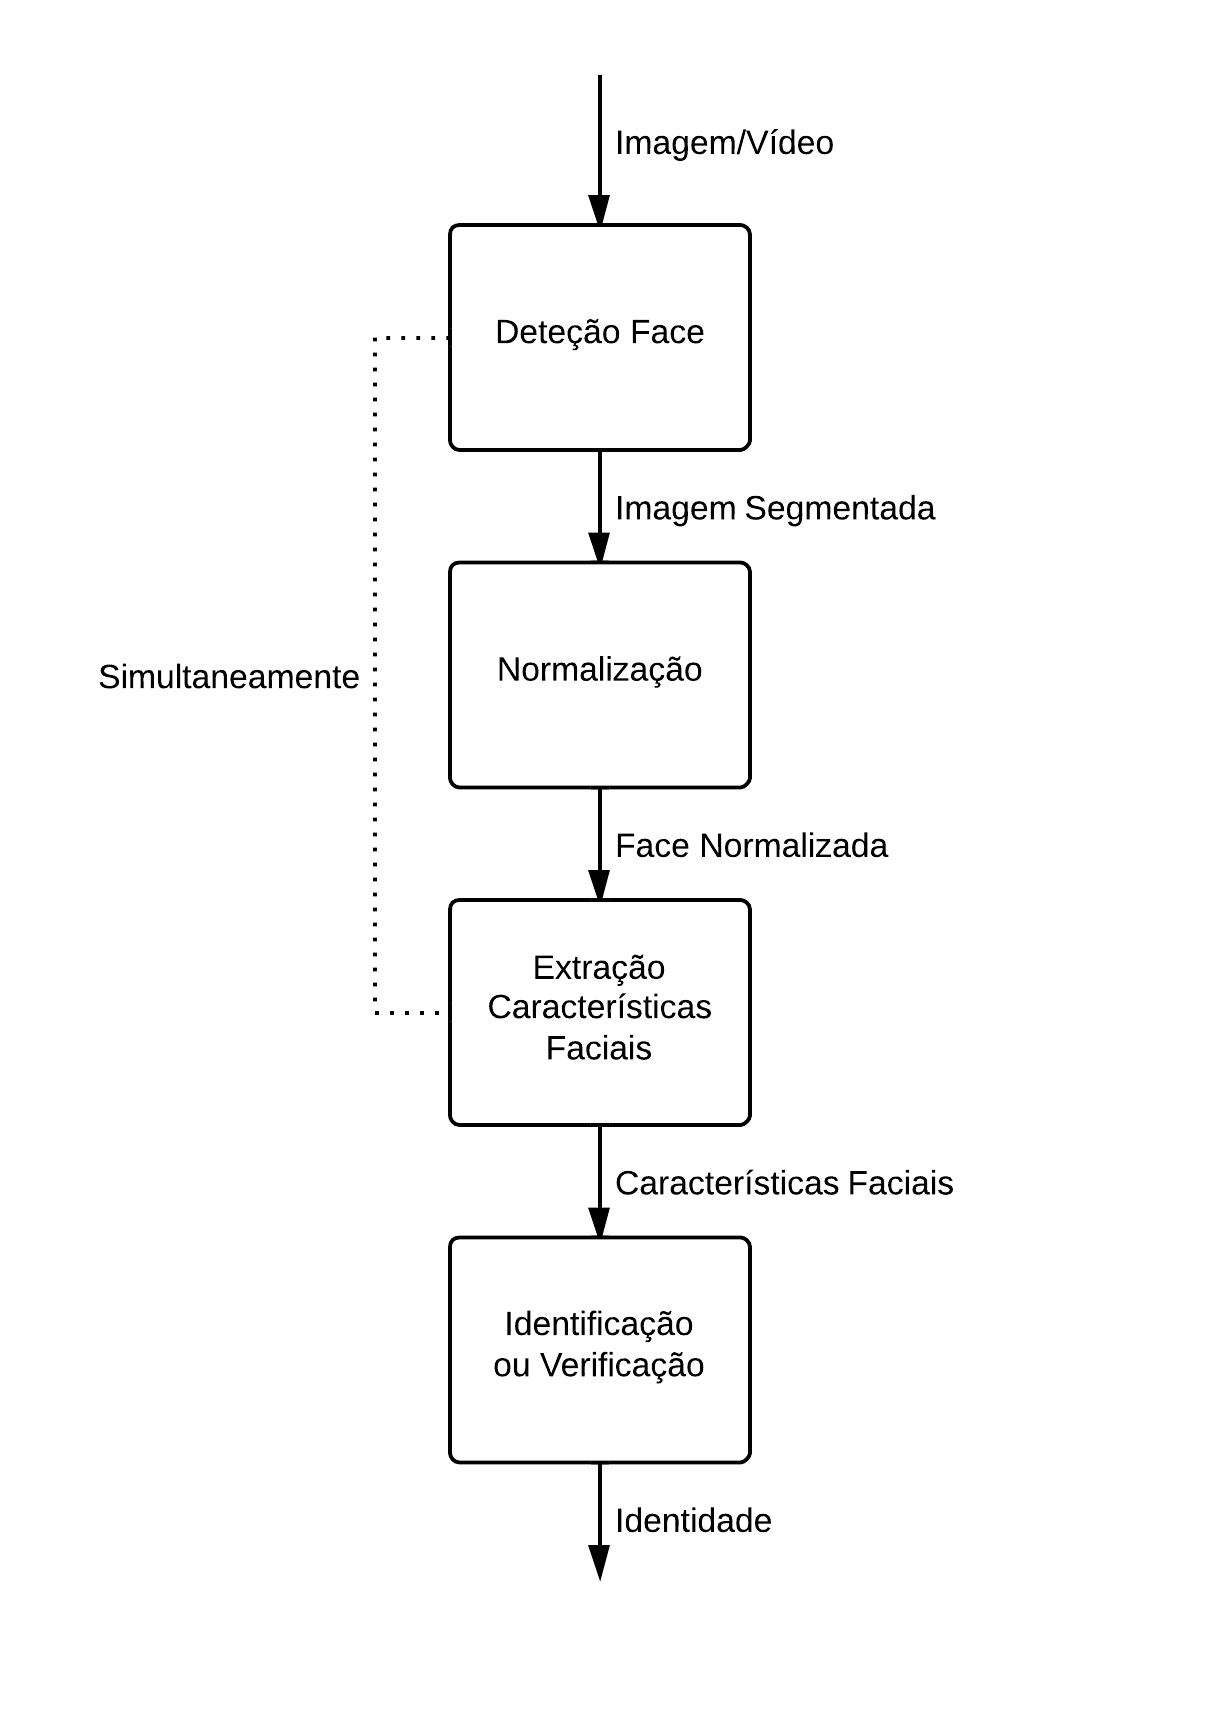
\includegraphics[width=0.5\textwidth]{SistemaGenericoRF}
    \caption{Sistema Genérico de Reconhecimento Facial}
    \label{fig:genericRF}
  \end{center}
\end{figure}

\subsection{Desafios} \label{desafios}
O reconhecimento facial automático em imagens é um problema complexo, sendo que existem um conjunto de desafios que se colocam na construção de um sistema de tipo. O primeiro passo em qualquer um desses sistemas, é a deteção de faces na imagem, a esse nível\textit{Yang et al.}, destacaram, no revisão ao estado da arte realizado em 2002,  os seguintes desafios \citep{Yang2002}:
\begin{itemize}
\item Pose e Orientação: A posição relativa da face à câmara pode sofrer uma grande variação dependendo do ambiente onde é capturada a imagem (variação no ângulo da face em relação à câmara vertical e horizontalmente, posição frontal, perfil). Ao variar a posição da face, alguns dos elementos que a permitem localizar e reconhecer podem ficar obstruídos. Avaliações efetuadas \citep{BlackburnDuaneM.;BoneMike;Phillips2001}, demonstram que este impacto é maior, quanto maior for o ângulo da pose em relação à posição frontal, sendo que uma variação até cerca de 25º não afeta significativamente os resultados do reconhecimento.
\item  Elementos Estruturais: a presença ou ausência de elementos estruturais, tais como barba ou óculos, assim como, a grande variação de forma e cor a que estes elementos podem apresentar afetam significativamente a forma como a face é percecionada pelo sistema.
\item Obstrução da face: as imagens captadas podem possuir objetos em frente à cara da pessoa a ser identificada, levando apenas a uma representação parcial da face na imagem.
\item Condições da imagem: aspetos como a resolução da imagem, o sensor utilizado para a captura e até mesmo eventuais defeitos associados à câmara utilizada podem potencialmente afetar o aspeto final da face na imagem.
\end{itemize}

Outro fator que afeta significativamente a perceção de uma face por um sistema de reconhecimento facial automático é a iluminação. Uma imagem pode ser capturada, com iluminação natural ou artificial. Para além disso, a iluminação pode estar sujeita a uma grande variação de tonalidades, intensidade e ângulo de incidência da luz.

Mesmo quando captadas pela mesma câmara, com as mesmas condições de iluminação e no mesmo local, podem existir variações significativas nas imagens captadas da face de uma pessoa devido às diferentes expressões faciais contidas nas imagens, fazendo com que este seja outro desafio a ultrapassar ao efetuar o reconhecimento facial automático.

O envelhecimento, ou eventuais alterações provocadas na face devido a fatores externos como por exemplo acidentes, exposição a condições extremas ou intervenção cirúrgica é outro dos fatores a ter em conta na identificação de uma pessoa.

Finalmente, existem ainda fatores como o elevado grau de semelhança entre pessoas com graus de parentesco próximos. Imagens capturadas de gémeos, ou até mesmo de pais e filhos, podem à primeira vista parecer imagens da mesma pessoa, tornando ainda mais difícil para um sistema automático efetuar a distinção dos indivíduos.

Assim sendo, para um reconhecimento fiável e eficaz é essencial que todas as etapas identificadas em \ref{sec:sub-problemas} sejam concluídas com sucesso. Sem uma correta deteção da presença de uma face na imagem, todos os passos subjacentes seriam impossíveis de ser realizados, por outro lado, o sucesso da extração das características faciais, encontram-se também dependente de uma normalização eficaz das imagens. No entanto, apesar desta dependência verificada entre as diversas etapas, cada uma delas representa problemas complexos, que devem a merecer a atenção e estudo de forma individual para que uma maior evolução das diversas técnicas envolvidas seja atingida \citep{Zhao2003}.


\section{Áreas de Aplicação}\label{sec:areasAplicacao}
O problema de reconhecimento facial automático tem merecido a atenção e estudo de inúmeros investigadores ao longo dos últimos 40 anos, motivados não só pelos desafios inerentes ao processo de reconhecimento facial, mas também pelas pela vasta gama aplicações onde a identificação de indivíduos é necessária \citep{Li2011}.

Adicionalmente, a evolução tecnológica da última década, permitiu a criação de sistemas computacionais mais poderosos, os quais tornaram possíveis desenvolvimentos na área que anteriormente seriam impensáveis gerando um ainda da maior interesse, tal como pode ser verificado pelo surgimento de uma vasta gama de aplicações comerciais e governamentais de reconhecimento facial, como é exemplo o sistema de fronteira automática dos aeroportos portugueses \citep{MinisteriodaAdministracaoInternaa}, assim como, pela recente aquisição de soluções de reconhecimento facial por parte de duas grandes empresas tecnológicas nomeadamente Google e Facebook.

De seguida encontram-se descritas, em cinco categorias, algumas das áreas de aplicação do reconhecimento facial automático, respetivamente ilustradas com exemplos de aplicação real. Esta categorização foi baseada no estudo efetuado em \cite{Li2011}, o qual é para nosso conhecimento o mais recente estudo efetuado às diversas áreas de aplicação do reconhecimento facial, assim como em estudos anteriores efetuados por \cite{Zhao2003}. Esta secção pretende apenas apresentar de uma forma sumária algumas das possíveis áreas de aplicação, e respetivas soluções, às quais o reconhecimento facial poderá ser aplicado, não pretendendo ser um estudo exaustivo de todas as soluções existentes.

\subsection{Controlo de Acesso e Segurança de Informação} \label{sec:controloAcesso}
A necessidade de sistemas de fácil utilização que assegurem a segurança da nossa informação digital, assim como da privacidade dos utilizadores, sem que para isso seja necessário a memorização e utilização de um sem número de palavras-chave e códigos de segurança é premente. Neste campo, o reconhecimento facial destaca-se ao permitir a criação de sistemas de autenticação não invasivos que requerem um nível de cooperação baixo por parte dos participantes, em contraste com os sistemas tradicionais como o uso de palavras-chave, ou mesmo de sistemas mais complexos como a análise de impressões digitais, retina ou íris. Por outro lado, este tipo de sistemas, permite ainda determinar a presença factual do utilizador que se pretende identificar, e não apenas determinar o conhecimento de um código de acesso à informação.

Atualmente, o uso de reconhecimento facial para o controlo de acesso a informação encontra-se já a ser utilizado em diversas aplicações comercias como são exemplos os sistemas de autenticação automática disponíveis numa grande variedade de computadores portáteis \ref{Asus, Hp, Topshiba}. De uma forma geral, nestes sistemas,o utilizador apenas necessita de se aproximar do computador para que o reconhecimento facial e consequente autenticação sejam efetuados. Desta forma o utilizador não necessita de efetuar qualquer intervenção para aceder aos seus dados ou de memorizar qualquer palavra-chave.

O uso de reconhecimento facial para garantir uma maior segurança de informação, ou efetuar um mais eficaz controlo do seu acesso, é geralmente aplicado em soluções com um número de utilizadores limitado e nas quais as imagens capturadas apresentam baixa variabilidade nas condições de iluminação e pose dos utilizadores. Desta forma, o nível de precisão do reconhecimento atingido nesta área é normalmente elevado, fazendo com que o nível de satisfação dos seus utilizadores seja também elevado \cite{Li2011}.

\subsection{Cartões Inteligentes e Identificação de Faces} \label{CartoesInteligentes}
Os documentos pessoais inteligentes registam uma presença cada vez mais ativa na sociedade atual, como é caso do cartão do cidadão português (CC), que à data de 5 de Novembro de 2012 já tinha sido adotado por mais de 7 milhões de portugueses \citep{Administrativa}, ou mesmo do passaporte eletrónico português (PEP), o qual recebeceu igualmente uma ampla aceitação desde a sua criação em 2006 \citep{MinisteriodaAdministracaoInterna}.

Tradicionalmente este tipo de documentos encontram-se dotados de capacidade de processamento e armazenamento próprios, podendo interagir com aplicações de terceiros como, por exemplo, sistemas de autenticação com recurso ao reconhecimento facial. O sistema designado de Reconhecimento Automático de Passageiros Identificados Documentalmente (RAPID)\citep{MinisteriodaAdministracaoInternaa}, desenvolvido pela empresa portuguesa Vision-Box \citep{Vision-Box} encontra-se desde 2007 em funcionamento nos vários aeroportos internacionais portugueses e tira partido das vantagens da associação da tecnologia de reconhecimento facial com documentos inteligentes. Em primeiro lugar, o sistema verifica se os dados armazenados no chip do passaporte são válidos, posteriormente, é efetuada uma comparação entre a fotografia armazenada no cartão e a imagem capturada do passageiro pelo dispositivo instalado na fronteira automática. Caso a identificação seja verificada, a porta que permite a passagem entre fronteiras é então automaticamente aberta. Todo o processo, encontra-se ainda a ser supervisionado por um operador numa cabine, o qual se encontra a supervisionar múltiplos dispositivos de identificação, sendo apenas necessária a sua intervenção quando não é efetuada uma identificação válida da pessoa.

O nível de precisão dos sistemas que tiram partido das sinergias entre cartões inteligentes e o reconhecimento facial apresenta uma correlação com o nível de atualização dos dados presentes nos documentos, sendo que  com um nível de atualização frequente é possível ser atingido um nível de satisfação elevado \cite{Li2011}, como se comprova pela bom funcionamento do sistema RAPID.
Contudo, esta é ainda uma área de investigação em aberto para que uma utilização destes sistemas de forma totalmente autónoma (sem que seja necessária a supervisão de um operador), em larga escala e, por exemplo, em ambientes não controlados seja possível.

\subsection{Entretenimento} \label{Entretenimento}
As tecnologias de reconhecimento facial apresentam uma forte potencialidade de aplicação nas área associadas ao entretenimento e à produção de conteúdos digitais, nomeadamente no que diz respeito à produção de jogo de computador e interação humano computador.

As consolas modernas estão dotadas de capacidade de processamento notáveis, para além disso, juntamente com estas consolas é cada vez mais comum o surgimento de dispositivos como o\textit{Kinect} da Microsoft que permitem novas formas de interação e a criação de novos tipos de jogos. Uma das novidades introduzidas pelo Kinect é a inclusão de diversos sensores e câmaras que permitem, entre outras coisas, efetuar um reconhecimento facial dos utilizadores. Desta forma, as equipas de desenvolvimento de jogos de computador, podem agora de uma forma mais fácil utilizar mecanismos de reconhecimento facial automático nos seus jogos de forma a criar jogos mais imersivos e personalizados. Este reconhecimento pode ainda ser aplicado ao nível da interação pessoa-computador  onde permite, a criação de sistemas com uma  uma maior facilidade de interação, uma vez que o próprio rosto poderá servir como um dispositivo de \textit{input} natural. 

À semelhança dos sistemas de controlo de acesso o reconhecimento facial automático na área do entretenimento é geralmente aplicado em soluções com um número de utilizadores limitado e onde o nível de precisão necessário não é muito alto fazendo assim com que a satisfação dos seus utilizadores seja, em geral, elevada.

\subsection{Gestão de Conteúdos Multimédia e Bases de Dados} \label{GestaoMultimedia}
A sociedade atual caracteriza-se pelo constante fluxo de informação a que os seus indivíduos se encontram expostos. A título de exemplo e de acordo com dados divulgados pela Intel\citep{IntelCorporation}, a cada minuto, são visualizados no Youtube 1,3 milhões de vídeos e carregadas para os seus servidores 30 novas horas de vídeo. Já o Flicker, no mesmo período de tempo, regista a visualização de 20 milhões de fotos e o carregamento de 3000 novas imagens para a sua plataforma. Segundo os mesmos dados, atualmente o número de dispositivos com ligação à Internet é equivalente ao da população mundial e é esperado que em 2015 seja o dobro dessa população.

Este crescimento verificado quer na quantidade de conteúdos produzidos, quer na diversidade de dispositivos que acedem a esses conteúdos, torna assim extremamente importante uma gestão e organização eficazes dos mesmos. Os métodos tradicionais de pesquisa e organização de conteúdos multimédia baseiam-se em anotações textuais associadas a estes conteúdos designadas de descritores. Com o uso de sistemas de reconhecimento facial é possível efetuar o reconhecimento das entidades presentes numa biblioteca multimédia mesmo que as suas fotografias não possuam qualquer anotação textual, uma vez que é feita uma análise da própria imagem e não apenas dos seus descritores, tornando-se assim um importante auxílio dos métodos tradicionais.

Atualmente existem no mercado diversas aplicações que permitem efetuar a organização de álbuns fotográficos  pessoais com recurso ao reconhecimento facial como por exemplo o Picasa da Google ou o iPhoto da Apple. Por outro lado, redes sociais como Google Plus e o Facebook, lançaram também recentemente serviços que permitem aos seus utilizadores a deteção e identificação automática de outros utilizadores presentes nas imagens carregadas para os seus servidores.

Apesar de a performance destes sistemas ter registado uma evolução notável nos últimos anos, a grande variabilidade associada às condições de captura de imagens e a grande quantidade de dados a ser processada faz com que exista ainda uma grande margem de evolução possível a este nível, sendo que a performance verificada ao nível do reconhecimento efetuado varia muito de acordo com a aplicação a analisar, assim como as características do conjunto de dados a organizar.

\subsection{Segurança e Aplicação da Lei} \label{sec:SegurancaAplicaçãoLei}
A preocupação com a segurança de instalações públicas e privadas, torna-se ainda mais premente em situações de grave crise económica como aquela que vivemos atualmente. Por outro lado, fatores como o controlo de emigração ilegal, preocupações relacionadas com a segurança de eventos com um grande impacto mediático ou mesmo o auxílio à investigação policial tornaram esta uma das áreas de aplicação que mais interesse despoletou por parte de sectores privados e governamentais desde o surgimento das primeiras tecnologias de reconhecimento facial.

Uma das aplicações mais comuns do reconhecimento facial em segurança é o reforço da vigilância da via pública. Desde 1998, diversas cidades implementaram sistemas de vigilância com recurso a reconhecimento facial, como são exemplos os sistemas instalados em \textit{Newham Borough of London}, \textit{Tampa (Florida)} e \textit{Virginia Beach (Virginia)} \citep{Li2011}.
Um outro exemplo, foi o sistema desenvolvido para os jogos olímpicos de 2008 em Pequim pela \textit{Chinese Academy Of Sciences} e que foi utilizado para validar as entradas nas cerimónias de abertura e encerramento dos jogos olímpicos \cite{ChineseAcademyOfSciences}.

A aplicação de sistemas de reconhecimento facial para a segurança e aplicação da lei tem atraído muita atenção por parte de sectores privados e governamentais, havendo o registo de alguns casos onde a sua aplicação se revelou um sucesso. Contudo, de uma forma geral estes sistemas debatem-se com um baixo nível de satisfação por parte dos seus utilizadores, isto porque, existe uma grande variabilidade nas condições de iluminação das imagens captadas, pose dos utilizadores, assim como, um número muito elevado de faces a analisar, resultando num número elevado de falsos positivos e consequentemente numa má performance dos sistemas \citep{Li2011}.

\section{Estratégias de Reconhecimento Facial}\label{sec:estratégias}
Após o trabalho inicial de Takeo Kanade em 1973 \citep{Kanade1973}, a área do reconhecimento facial automático passou um período de dormência até meados da década de 90, onde os trabalhos realizados recorrendo a métodos como \textit{Principal Component Analysis (PCA)}, \textit{Linear Discriminant analysis (LDA)} e \textit{Ellastic Grapth Matching (EGM)}, revitalizaram a área \citep{Chellappa2010}. Ao nível da PCA, o método
 \textit{Eingenfaces} desenvolvido por Turk e Pentland em 1991 \cite{Turk1991}, foi um marco fundamental no rejuvenescimento do reconhecimento facial automático. Este método tira partido da redundância natural existente entre as representações faciais de diversos indivíduos, para através de uma análise dos componentes principais das faces, desenvolvida anteriormente por Kirby e Sirovich  \cite{Kirby1990}, efetuar uma representação de baixo nível das faces existentes. Posteriormente, o método \textit{Fisherfaces} \cite{Belhumeur1997, Etemad1997, Zhao1998}, que tira partido da aplicação de LDA após uma análise inicial dos componentes principais da imagem, apresentou também resultados positivos em experiências em bases de dados com um número elevado de faces a analisar. Finalmente, ao nível de EGM, foi percursor o trabalho realizado por Wiskott \textit{et al.} \cite{wiskott1997face}. 
 
Desde então, diversos investigadores estenderam estes três tipos de algoritmos. Em 2003, Zhao \textit{et al.} \citep{Zhao2003} efetuaram um estudo aprofundado das técnicas desenvolvidas até então classificando-as em três categorias. Métodos holísticos, caso estes usem toda a região da face como fonte de comparação no reconhecimento, métodos baseados nas caraterísticas faciais, caso estes usem as características extraídas como informação essencial para a classificação da face e ainda como híbridos, caso seja utilizada uma mistura de ambos os métodos. Os resultados desta classificação podem ser visualizados na tabela \ref{tabelaZhao}.

\begin{center}
\begin{table}
	\caption{Categorização dos Métodos de Reconhecimento Facial em Imagens por Zhao \textit{et al.} \citep{Zhao2003}}
	% title of Table
	\centering
	% used for centering table
	\begin{tabular}{l p{8cm}}
	% centered columns (4 columns)
	\hline\hline
        Método                     & Trabalho Representativo\\
	% inserts table
	%heading
	\hline
		% inserts single horizontal line
Holistic methods	 \\	
$\quad$ \textit{Principal Component analysis (PCA)} \\
$\qquad$  Eigenfaces                 & Direct application of PCA [Craw and Cameron 1996; Kirby and Sirovich 1990; Turk and Pentland 1991] \\
$\qquad$        Probabilistic eigenfaces   & Two-class problem with prob. measure [Moghaddam and Pentland 1997] \\
$\qquad$        Fisherfaces/subspace LDA   & FLD on eigenspace [Belhumeur et al. 1997; Swets andWeng 1996b; Zhao et al. 1998] \\ 
$\qquad$        SVM                        & Two-class problem based on SVM [Phillips 1998] \\ 
$\qquad$        Evolution pursuit          & Enhanced GA learning [Liu andWechsler 2000a] \\ 
$\qquad$        Feature lines              & Point-to-line distance based [Li and Lu 1999] \\ 
$\qquad$        ICA                        & ICA-based feature analysis [Bartlett et al. 1998] \\ 
$\quad$ \textit{Other Representations} \\
$\qquad$        LDA/FLD                    & LDA/FLD on raw image [Etemad and Chellappa 1997] \\ 
$\qquad$        PDBNN                      & Probabilistic decision based NN [Lin et al. 1997] \\

Feature-based methods \\
$\qquad$        Pure geometry methods      & Earlier methods [Kanade 1973; Kelly 1970]; recent methods [Cox et al. 1996; Manjunath et al. 1992] \\ 
$\qquad$        Dynamic link architecture  & Graph matching methods [Okada et al. 1998;Wiskott et al. 1997] \\ 
$\qquad$        Hidden Markov model        & HMM methods [Nefian and Hayes 1998; Samaria 1994; Samaria and Young 1994] \\

Hybrid methods \\
$\qquad$        Convolution Neural Network & SOM learning based CNN methods [Lawrence et al. 1997] \\ 
$\qquad$        Modular eigenfaces         & Eigenfaces and eigenmodules [Pentland et al. 1994] \\ 
$\qquad$        Hybrid LFA                 & Local feature method [Penev and Atick 1996] \\ 
$\qquad$        Shape-normalized           & Flexible appearance models [Lanitis et al. 1995] \\ 
$\qquad$        Component-based            & Face region and components [Huang et al. 2003] \\
        \hline
    \end{tabular}
	\label{tabelaZhao}
\end{table}
\end{center}
 
 Tal como referido na secção \ref{desafios} deste relatório, o reconhecimento facial é uma tarefa complexa, composta por um conjunto de sub-problemas que enfrentam uma série de desafios para a sua conclusão. O primeiro desafio em qualquer sistema de reconhecimento facial é a deteção da face na imagem, a esse nível o trabalho realizado por Paul Viola e Michael Jones \citep{Viola2004} é considerado como um dos mais robustos métodos disponíveis na atualidade. Outras áreas onde a investigação atual se encontra focada têm a ver com a criação de métodos de reconhecimento facial robustos em relação à iluminação das imagens, assim como a pose dos indivíduos representados. \citep{Chellappa2010}.
 
 Ao nível da pose, o uso de  \textit{3D morphable face models} \cite{Blanz2003} tem revelado resultados positivos em posições não frontais. Estes algoritmos simulam o processo de formação de uma face em 3D, estimando a sua representação tridimensional a partir de imagens 2D fornecidas ao sistema com recurso a técnicas de computação gráfica. Esta estimativa é efetuada através do encaixe de um modelo 3D de faces na própria imagem fornecida, modelo esse apreendido através da digitalização 3D de um conjunto de rostos e respetiva textura. No entanto, em grande parte dos modelos desenvolvidos a seleção manual de um pequeno número de características faciais é requerida e o poder de computação necessário para a criação dos modelos é elevado. Extensões destes modelos foram também propostas para criar sistemas mais robustos em relação à variação na iluminação.  
 
 Outras abordagens que têm em vista a criação de sistemas de reconhecimento facial robustos em relação à iluminação centram os seus esforços na estimação do albedo para a normalização das imagens. O albedo representa a relação entre a quantidade de luz refletida por um ponto e quantidade de luz incidente, métodos recentes centram-se no desenvolvimento de filtros estocásticos não estacionários para a estimação de mapas de albedo das amostras faciais \cite{Biswas2009}. Estes mapas podem ainda ser combinados com os modelos 3D faciais desenvolvidos para uma representação facial mais completa. Apesar de os resultados obtidos por estes métodos serem promissores quando comparados com os métodos tradicionais como o \textit{Eigenfaces}, estes métodos ainda carecem de maior validação, uma vez que as suas avaliações foram feitas utilizando conjuntos de dados controlados e de reduzida dimensão \citep{Chellappa2010}.
 
O investimento realizado na investigação de metodologias de reconhecimento facial automático tem permitido progressos notáveis na área. Do mesmo modo, a investigação em áreas relacionadas como a deteção de faces nas imagens, o envelhecimento facial ou o reconhecimento de expressões faciais em imagens tem permitido evoluir ainda os resultados obtidos. Devido à complexidade envolvida no processo de reconhecimento facial automático a evolução na área encontra-se assim intrinsecamente ligada à evolução verificada nas múltiplas áreas envolvidas, sendo que a investigação independente de cada uma é crítica para uma resolução eficaz da grande variabilidade de desafios que o reconhecimento facial automático se propõe ultrapassar.

\subsection{Soluções Existentes}\label{sec:soluções}
A investigação desenvolvida nos vários centros de investigação na década de 90, levou à passagem das soluções de reconhecimento facial automático de meros protótipos de laboratório, para soluções comerciais de elevado valor acrescentado, dessas soluções resultaram três categorias comerciais de produtos na área do reconhecimento facial:
\begin{itemize}
\item Soluções Completas. Estas soluções caracterizam-se por oferecer toda a infraestrutura necessária para efetuar o reconhecimento facial, quer a nível de software, quer a nível de hardware.
\item Software. Soluções tradicionais de sistemas de reconhecimento facial, que consistem em software que permite efetuar o reconhecimento facial independentemente do hardware utilizado para a captura de informação.  Dentro destas soluções existe uma grande variedade nos produtos oferecidos, desde soluções baseadas na captura de imagens 2D estáticas, imagens 3D e vídeo. Para além disso, as soluções oferecidas encontram disponíveis para serem utilizadas em diversas plataformas, como por exemplo dispositivos móveis ou através da Internet.
\item SDK para reconhecimento facial. Permitem aos clientes, através de módulos independentes ou APIs, a criação de novas aplicações de reconhecimento facial.
\end{itemize}

Para além do reconhecimento facial automático, as soluções disponíveis possuem muitas vezes também associados outros métodos de biometria, como por exemplo reconhecimento de íris ou impressões digitais, assim como métodos mais tradicionais de autenticação como o uso de cartões de identificação ou passwords, de modo a aumentar a robustez e segurança dos sistemas.

Na tabela \ref{tab:solucoesExistente}, encontram-se listadas algumas das soluções comerciais atualmente existentes de reconhecimento facial, assim como alguns exemplos de aplicações onde estas foram utilizadas. Esta tabela não pretende representar um levantamento exaustivo das soluções existentes mas apenas ilustrar a vasta gama de produtos disponíveis.

Para além das soluções comerciais de reconhecimento facial ao longo dos últimos anos surgiram também algumas soluções gratuitas de reconhecimento facial. Deste tipo de soluções são exemplo o software Picasa da Google, ou software iPhoto da Apple que permitem aos seus utilizadores a organização de álbuns multimédia com recurso ao reconhecimento facial. Por outro lado, redes sociais como Google Plus e o Facebook, lançaram também recentemente serviços que permitem aos seus utilizadores a deteção e identificação automática de outros utilizadores presentes nas imagens carregadas para os seus servidores.


\section{Análises de Desempenho Efetuadas}\label{sec:performance}
A performance de um sistema de reconhecimento facial depende de uma grande variedade de fatores como a iluminação, posição da face na imagem, expressão facial e presença ou ausência de adereços (ex:óculos). Por outro lado, as condições de utilização do próprio sistema, tais como o número de utilizadores diferentes e a frequência de utilização, são também fatores a ter em conta ao avaliar a performance de um sistema. Uma avaliação apropriada dos sistemas de reconhecimento facial encontra-se então dependente da existência de uma base de dados de grandes dimensões e consequentemente um conjunto de casos de teste vasto, assim como, da existência de métodos apropriados para essa avaliação.

A criação do programa FERET em 1993, pelo NIST, permitiu assim colmatar uma lacuna existente na avaliação dos sistemas de reconhecimento facial existentes com a criação de uma base de dados de faces de grande dimensões assim como de um protocolo de avaliação dos respetivos sistemas de reconhecimento facial. Com base no protocolo desenvolvido foram levadas a cabo avaliações aos nos anos de 1994 e 1995. Um novo protocolo foi criado para a avaliação realizada em 1996. Posteriormente, o mesmo instituto realizou novas avaliações baseadas no protocolo FERET96 na edição de 2000 dos FRVT, a partir de 2002, um novo protocolo foi criado (protocolo FRVT 2002), com base no protocolo FERET96, mas com a particularidade de permitir a avaliação de sistemas de biometria em geral e não apenas sistemas de reconhecimento facial. Com base no novo protocolo criado foram então realizadas avaliações nos anos de 2002, 2006 e 2010. A decorrer encontram-se ainda as avaliações FRVT 2012. 

As avaliações levadas a cabo durante os programas FERET e FRVT constituem desta forma uma boa base para a análise da evolução dos sistemas de reconhecimento facial automático ao longo dos últimos 20 anos, tal como pode ser visto na figura \ref{fig:evolucaoAvaliacoes}. De seguida encontram-se descritas os principais objetivos e conclusões retiradas dos programas FERET e FRVT:

\subsection{FERET}
Para além dos objetivos anteriormente citados de criação de uma base de dados de grandes dimensões e de criação de um protocolo que permitisse uma avaliação concreta e de base científica dos algoritmos existentes, o programa FERET tinha ainda como propósitos avaliar o estado da arte e identificar futuras áreas de desenvolvimento do reconhecimento facial \cite{Phillips2000}. Tendo em conta estes objetivos, foi então avaliada a performance dos diferentes algoritmos em diferentes cenários, categorias de imagens e diferentes versões dos próprios algoritmos. A performance foi computada para situações de identificação e verificação de faces, estando os principais resultados da última avaliação, efetuada em 1996, descritos em Phillips \textit{et al.} \cite{Phillips2000}.

A primeira avaliação do programa FERET, em 1994, consistia num três de conjuntos de testes, cada um com uma galeria e conjunto de provas diferentes. O primeiro conjunto, consistia numa prova de reconhecimento de faces de uma galeria de 316 faces. O segundo, tinha com objetivo determinar a capacidade dos algoritmos de rejeitar faces não presentes na galeria, designadas de falso-alarme. O terceiro, tinha como objetivo analisar os efeitos da pose na performance dos algoritmos \citep{Phillips2000}.

Em 1995, teve lugar a segunda avaliação, com o objetivo de  avaliar os mesmo algoritmos em galerias de maior dimensão. A performance foi medida num único teste, com uma galeria de 817 indivíduos conhecidos, tendo sido dado um maior ênfase na avaliação de provas duplicadas. Um duplicado é uma imagem cuja imagem correspondente da galeria foi geralmente capturada em dias diferentes  \citep{Phillips2000}.

Na última edição, em 1996, e já com um protocolo atualizado, foram testados 12 algoritmos de reconhecimento facial, e estudada a sua performance em quatro situações diferentes, usando para isso uma galeria com um total de 1196 indivíduos. Na primeira situação, a galeria e as imagens de prova foram tiradas no mesmo dia e sobre as mesmas condições de iluminação. No segundo conjunto de provas, a galeria e as imagens de prova foram tiradas em dias diferentes. Para o terceiro teste, a galeria e as respetivas provas foram capturadas com pelo menos um ano de diferença. Finalmente, no quarto e último conjunto de testes, a galeria e as imagens de prova forma tiradas no mesmo dia, mas com diferentes condições de iluminação.

Várias conclusões foram retiradas das avaliações efetuadas. A primeira conclusão foi que, de facto, se verificava uma evolução nas técnicas de reconhecimento facial, uma vez que os resultados foram progressivamente melhores, mesmo quando comparadas versões diferentes do mesmo algoritmo. Essa conclusão é suportada pela análise dos resultados do caso geral de identificação, testado em todas as edições, onde as imagens da galeria e da prova foram capturadas no mesmo dia e com a mesma iluminação. Nesse teste em 1994, apenas 78\% indivíduos foram identificados com sucesso numa galeria de 317 indivíduos, ao passo que em 1995 foram identificados já 93 \% dos indivíduos numa galeria de 831 e nos testes da última edição (1996), 95\% dos indivíduos foi identificado numa galeria de 1196 indivíduos. De igual forma, foi também verificada evolução na deteção de duplicados, mantendo-se no entanto as percentagens de identificação de duplicados mais reduzidas quando comparadas com o caso geral de identificação devido à maior complexidade do problema.

Outra conclusão retirada foi que a performance se encontra dependente da galeria e conjunto de imagens de prova utilizadas, uma vez que foi verificado que mudando a galeria, mas mantendo o mesmo tipo de teste a ser efetuado a percentagem de indivíduos identificados varia significativamente. Para a galeria e conjunto de prova capturadas no mesmo dia a percentagem varia entre os 80\% e os 94\%, enquanto que para galeria e conjunto de prova, capturadas em dias diferentes essa percentagem varia entre os 24\% e os 69\% porcento. Para além disso, não se existiu qualquer algoritmo que se revelasse superior em todas as quatro situações de teste realizadas em 1996, variando as performances, conforme a situação de teste.

Finalmente, conforme a tarefa a efetuar, identificação ou verificação de faces, ficou também demonstrado que não havia uma técnica que se superiorizasse em ambas as situações, comprovando que o reconhecimento facial é uma tarefa complexa que necessita de um estudo e investigação concretos tendo em conta a área de aplicação em vista.

\subsection{FRVT}
Durante a década de 90 registou-se um progresso assinalável nas diversas técnicas de reconhecimento facial, tendo para isso sido muito importante o papel desempenhado por iniciativas como o FERET. No final da década de 90, assistiu-se então a uma passagem dos sistemas de reconhecimento facial existentes de meros protótipos universitários, para aplicações comerciais de reconhecimento facial automático, tal como pode ser comprovado  pela participação de 5 soluções comerciais na primeira edição dos \textit{Facial Recognition Vendor Test}, no ano 2000. Esta avaliação, tinham como objetivo maioritário efetuar uma avaliação técnica das capacidades dos sistemas comerciais de reconhecimento facial disponíveis, de forma a compreender os pontos fortes e fracos de cada sistema, obtendo também uma análise do estado da arte do reconhecimento facial à data \cite{BlackburnDuaneM.;BoneMike;Phillips2001}. Estas avaliações foram ainda repetidas em 2002, 2006, 2010 e ainda em 2012.

A primeira edição dos FRVT, em 2000, utilizou o mesmo protocolo de avaliação da avaliação última avaliação FERET em 1996, no entanto, os testes efetuados eram significativamente mais exigentes do que a avaliação anterior, sendo utilizada também uma muito maior variedade de imagens. Os resultados da avaliação efetuada foram ser reportados para as seguintes oito categorias: compressão, distância, expressão,  media, iluminação, pose, resolução e variação temporal. Ao nível das conclusões retiradas, podem ser destacados os seguintes tópicos \cite{BlackburnDuaneM.;BoneMike;Phillips2001, Chellappa2010, Li2011}:
\begin{itemize}
\item Compressão de imagens, utilizado JPEG, até 40:1 não reduziu a taxa de reconhecimento;
\item Pose não afeta o reconhecimento de forma significativa até $\pm$ 25º, mas afeta significativamente quando são atingidos os $\pm$ 40º;
\item De forma equivalente ao registado no programa FERET, o uso de diferentes iluminações interiores não afeta significativamente os resultados obtidos, no entanto esses resultados são afetados caso haja uma mudança entre zonas interiores e exteriores;
\item Registou-se uma melhoria significativa dos resultados obtidos em imagens tiradas com mais de 18 meses de distância, quando comparado com os resultados obtidos no FERET. (Aumento de 5\% a 12\% de faces identificadas conforme o conjunto de dados avaliado).
\end{itemize}

A segunda edição dos FRVT teve lugar em 2002, contou com a participação de soluções de reconhecimento facial de 10 empresas distintas. Esta edição consistiu em duas provas fundamentais, os \textit{High Computational Intesity test (HCInt)} e os \textit{Medium Computational Intensity test (MCInt)}. Os HCInt tinham como objetivo medir a performance dos sistemas existentes em 121 589 imagens frontais de 37 435 pessoas, representando um desafio computacional de elevado grau de exigência, como comprovado pelas 242 horas de computação necessárias para efetuar os testes. Os \textit{Medium Computational Intensity test (MCInt)}, assemelhavam-se às medições efectuadas em avaliações anteriores, como o FERET e o FRVT 2000, tendo como objetivo medir a performance dos sistemas em imagens de diferentes categorias, nomeadamente não frontais, capturas no interior e exterior, entre outros. As conclusões retiradas desta avaliação foram as seguintes \cite{Chellappa2010, Li2011}:
\begin{itemize}
\item Melhores sistemas são insensíveis a variações de luz interior;
\item Reconhecimento facial em imagens exteriores é ainda um desafio por resolver;
\item Utilização de \textit{3D morphable models} melhora a performance em situações não frontais;
\item Características como sexo e idade podem afetar significativamente a performance, sendo que se registou maior facilidade em distinguir homens e pessoas com idade superior.
\item O tempo de captura entre provas afeta significativamente a performance, registando-se uma diminuição linear da performance com o aumento do tempo.
\end{itemize}

As últimas edições dos FRVT para as quais foram divulgados resultados foram as edições de 2006 \cite{Phillips2007} e a de 2010. Na edição de 2010 a competição não assumiu o nome de FRVT 2010, mas sim de \textit{Multiple Biometric Evaluation (MBE)} 2010-\textit{still image track}, uma vez que além de avaliados sistemas de reconhecimento facial automático foram também avaliados sistemas de biometria com base na análise da íris. \cite{Grother2010}. Foi também realizada uma edição dos FRTV em 2012, mas a avaliação dos sistemas ainda se encontra a decorrer, não havendo por isso resultados divulgados.

\begin{figure}[t]
  \begin{center}
    \leavevmode
    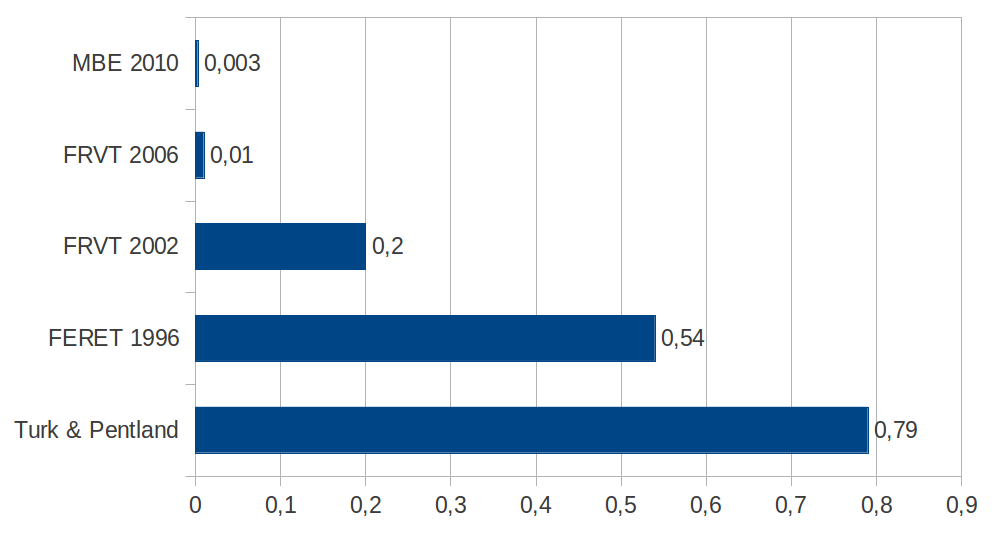
\includegraphics[width=0.9\textwidth]{EvolucaoAvaliacoes}
    \caption{A redução da taxa de erro para os algoritmos estados da arte tal como documentado nas avaliações FERET, FRVT 2002, FRVT 2006 e MBE 2010 \cite{Phillips2007, Grother2010}}	
    \label{fig:evolucaoAvaliacoes}
  \end{center}
\end{figure}

Em 2006, foi analisada a performance de sistemas de reconhecimento facial, de 22 organizações e de 10 países diferentes, baseados em representações 3D e em imagens estáticas de faces. As avaliações consistiam em três testes distintos: comparação de imagens capturadas com luz interior; comparação de digitalizações de faces 3D com base na forma e textura; comparação de imagens capturadas em estúdio com imagens capturadas em corredores e átrios. Em 2010, para além do conjunto de dados analisados em 2006 e 2002, de modo a averiguar a evolução comparativa dos algoritmos, foi também analisado um segundo conjunto de imagens recolhidas por várias agências de segurança e compiladas pelo \textit{Federal Bureau of Investigation (FBI)}. Este segundo conjunto de dados possuía mais de 1 milhão de faces fazendo da avaliação de 2010 a avaliação em maior escala feita aos sistemas de reconhecimento facial à data. Das provas de 2006 e 2010, as principais conclusões obtidas foram as seguintes \cite{Phillips2007, Grother2010, Chellappa2010, Li2011}:
\begin{itemize}
\item Desde 1993 foram atingidas melhorias de 2 ordens de magnitude;
\item Os resultados de 2010 e 2002 mostram uma melhoria de 1 ordem de magnitude nos sistemas de reconhecimento facial (Para um \textit{false accept rate (FAR)} de 0.001, foi registado em 2002 um \textit{false reject rate (FRR)} de 0.2, enquanto que em 2010 FRR=0.038);
\item Em condições de captura de informação controlada, a performance medida de sistemas de reconhecimento facial e sistemas baseados na análise da íris foi equivalente;
\item A performance de sistemas baseados em imagens estáticas e sistemas baseados em representações 3D da face foi equivalente;
\item Iluminação e resolução das imagens representam um papel fundamental no reconhecimento facial;
\end{itemize}
\chapter{Abstração de Imagens} \label{chap:abstracao} - TO-DO
A abstração de imagens permite uma simplificação do conteúdo visual ao retirar informação redundante e dar destaque apenas à informação essencial representada. Desta forma, os artistas têm a capacidade  de guiar a atenção de quem visualiza a imagem para conteúdos específicos, influenciando assim a perceção da mesma e tornado a comunicação mais eficaz.

Este filtros permitem uma simplificação do conteúdo visual ao retirar informação redundante e destacando a apenas a informação essencial. Estes filtros são tradicionalmente utilizados por artistas para comunicar de uma forma mais eficaz a informação pretendida ao retirar a informação desnecessária de imagens foto-realistas \citep{Kyprianidis2009}.


\section{Resumo ou Conclusões}

\chapter{Perspectiva de Solução} \label{chap:solução}

O reconhecimento facial em imagens sofreu uma evolução notável nos últimos 20 anos, tal como documentado no capítulo \ref{chap:reco} deste relatório. 

Em cenários cooperativos com condições de captura de imagens controladas, nomeadamente ao nível da pose, iluminação e expressões faciais, considera-se mesmo que o problema de verificação 1:1 se encontra praticamente resolvido, uma vez que as taxas de reconhecimento atingidas são satisfatórias para a grande maioria das aplicações \citep{Li2011}. Existem também várias aplicações em situações reais com um bom nível de satisfação por parte dos seus utilizadores, como é o caso do sistema de fronteira automático dos aeroportos portugueses (ver \ref{CartoesInteligentes}), ou o controlo de entradas nas cerimónias inaugurais dos jogos olímpicos de Pequim (ver \label{Vigilancia}). Em condições específicas e favoráveis, é então possível considerar que os sistemas de reconhecimento facial automático atuais conseguem mesmo ultrapassar a capacidade de reconhecimento humana, uma vez que conseguem identificar com precisão um maior número de faces do que aquelas que um humano consegue.

Contudo, o problema de reconhecimento facial automático ainda se encontra longe de ser um problema totalmente resolvido. Em cenários onde é registada uma grande variação ao nível da pose, iluminação ou outros fatores identificados na secção \ref{desafios} deste relatório, a identificação das entidades capturadas é ainda uma tarefa desafiante  \citep{Li2011}. Para além disso, a performance e satisfação obtida por parte dos utilizadores dos sistemas atuais demonstra uma grande variação tendo em conta as situações onde estes sistemas são utilizados. 

Por outro lado, a crescente ubiquidade tecnológica e poder computacional presente nos diversos dispositivos utilizados no nosso dia a dia, aumenta o leque de aplicações possíveis do reconhecimento facial automático, apresentando novos desafios às soluções de atualmente existentes.(ver \label{sec:areasaplicacao})

Assim sendo, torna-se pertinente a continuação da investigação na área do reconhecimento facial em imagens. Para além disso, o elevado valor comercial das soluções existentes e consequente falta soluções abertas permite alcançar uma boa visibilidade dos resultados obtidos.

Ao nível da abstração de imagens, estudos efetuados demonstraram que aplicação destes filtros na recuperação de informação multimédia, nomeadamente no âmbito da da ilustração automática de texto têm a potencialidade de melhorar a informação retornada, assim como reduzir significativamente as necessidades de processamento e armazenamento das imagens \citep{Coelho2012}. 

Tendo em conta a importância e a necessidade de investigação na área do reconhecimento facial automático, e uma vez que não existem estudos relativos à utilização de filtros de abstração no processo de reconhecimento facial, torna-se pertinente o estudo do seu impacto, no âmbito desta dissertação. Desta forma, a hipótese levantada no âmbito desta dissertação é então que o uso de a abstração em imagens que vão ser ser alvo de reconhecimento facial pode melhorar a o processo de reconhecimento facial automático em imagens.

\section{Objetivos} \label{sec:objetivosperpectiva}
O principal objetivo deste projeto visa o estudo do impacto de filtros de abstração visual de informação no processo de reconhecimento facial automático em imagens. Para isso, destacam-se o seguinte conjunto de objetivos parciais:

\begin{enumerate}
\item Desenvolvimento de um sistema de reconhecimento facial de personalidades;
\item Integração da abstração de imagens no sistema desenvolvido;
\item Avaliação dos resultados da abstração de imagens no processo de reconhecimento facial;
\end{enumerate}

Da avaliação efetuada, para além da publicação desta dissertação, espera-se ainda a publicação de um artigo científico onde sejam descritos os resultados obtidos.

\section{Implementação} \label{sec:implementacao}

Uma vez que não se pretende no âmbito desta dissertação efetuar investigação ao nível dos algoritmos de reconhecimento facial, mas sim ao nível do impacto do uso de imagens abstraídas nesse sistemas, a implementação desses algoritmos terá por base a utilização de soluções abertas de reconhecimento facial, nomeadamente a biblioteca \textit{Open CV (Open Source Computer Vision)}.

Ao nível dos filtros de abstração o estudo será efetuado utilizado o filtro \textit{Anisotropic Kuwahara}.
Este filtro foi utilizado anteriormente, e com resultados positivos, em abstração de imagens para a recuperação de informação multimédia, pelo que se considera adequada a sua utilização no âmbito deste projeto.

Por último, ao nível das coleções de dados a analisar, temos em vista a utilização de duas coleções a primeira é a uma coleção standard, chamada \textit{Labeled Faces in the Wild} e que permite obter resultados comparativos com avaliações efetuadas anteriormente a sistemas de reconhecimento facial existentes. A segunda é a coleção de imagens Sapo Fama, qual agrega uma base de dados de imagens de personalidades famosas nacionais e internacionais, representado uma possível área de aplicação do sistema desenvolvido.
	
\subsection{Sistema de Reconhecimento Facial Base - OpenCV Face Recognizer}
O \textit{OpenCV} é uma biblioteca de código aberto nas áreas de visão por computador e \textit{machine learning}, onde se encontra disponível a implementação de mais de 2500 algoritmos. Esta biblioteca possui uma comunidade de mais de 47 mil pessoas, já registou mais de 5 milhões de downloads e é utilizada globalmente por empresas como a Google, Yahoo, Microsoft, Intel, IBM, Sony, Honda, Toyota \cite{Team}. 

Ao nível do reconhecimento facial, esta biblioteca disponibiliza um módulo denominado \textit{Face Recognizer}, onde se encontram implementados os algoritmos \textit{Eigenfaces}, \textit{Fisherfaces} e \textit{Local Binary Patterns Histograms}.

Tendo em conta a ampla utilização da biblioteca OpenCV e a sua constante atualização pela comunidade, assim como as facilidades providenciadas pelo módulo de reconhecimento facial, esta foi considerada a biblioteca ideal para utilizar como base de implementação do sistema de reconhecimento facial a criar. De seguida encontram-se brevemente descritos os três algoritmos implementados no módulo \textit{Face Recognizer:}

\subsubsection{Eigenfaces}
O método \textit{Eigenfaces} foi introduzido por \cite{Belhumeur1997} e tira partido da Análise dos Componentes Principais (ACP) para efetuar o reconhecimento facial automático.

A análise de componentes principais tem como objetivo determinar as relações existentes entre diferentes conjuntos de dados, nomeadamente ao nível das suas diferenças e semelhanças, tirando partido da redundância existente para criar uma representação reduzida dos dados sem que a perda de informação ocorrida seja significativa. As imagens faciais possuem uma grande redundância natural, o algoritmo \textit{Eigenfaces}, através da análise dos componentes principais dessas imagens, efetua uma projeção das imagens faciais num sub-espaço onde se evidenciam apenas as variações entre as diversas caras conhecidas pelo sistema.

A redução do espaço de representação revela-se fulcral no problema de reconhecimento facial em imagens, devido à grande dimensionalidade exigida para a representação de uma face. Considerando, por exemplo, uma dada imagem de $n$x$m$ \textit{pixels} de tons cinzentos, essa imagem poderia ser traduzida por um espaço vetorial de $m = $ $n$x$m$ \textit{pixels}, assim sendo, uma imagem de apenas $256x256$ \textit{pixels} necessitaria de um total de $65536$ \textit{pixels} para ser representada.

O processo de reconhecimento facial com recurso ao algoritmo \textit{Eigenfaces} consiste então nos seguintes passos:
\begin{enumerate}
\item Aquisição de um conjunto de dados iniciais (conjunto de treino);
\item Projeção dos dados obtidos num sub-espaço de faces através da ACP;
\item Aquisição de uma imagem a reconhecer;
\item Projeção da face a reconhecer no sub-espaço do conjunto de treino, calculando as distâncias obtidas para cada face conhecida pelo sistema;
\item Determinar qual a face do conjunto de treino com menor distância à face a reconhecer;
\item Caso a distância para a face obtida seja menor do que um limite operacional estabelecido, a imagem é reconhecida como sendo essa pessoa, caso contrário, a face é identificada como sendo uma pessoa desconhecida pelo sistema.
\end{enumerate}

Este método efetua assim uma abordagem holística ao problema de reconhecimento facial em imagens, uma vez que tem em consideração a representação facial como um todo, não fazendo a distinção entre pontos específicos da face como olhos, orelhas ou nariz para efetuar o reconhecimento facial. Uma vantagem deste tipo de representação é a reduzida sensibilidade ao ruído presente nas imagens \cite{Zhao2003}.

\subsubsection{Fisherfaces}
A análise dos componentes principais visa determinar o sub-espaço onde se verifica uma maior variação entre um conjunto de imagens, no entanto, a variação na representação facial de uma pessoa encontra-se muitas vezes relacionada com mudanças de expressões faciais ou iluminação dos indivíduos. Assim sendo, o sub-espaço criado pelo algoritmo \textit{Eigenfaces} não traduz muitas vezes as apenas as diferenças de identidade entre os diversos indivíduos, mas também as diferenças verificadas ao nível das condições de captura das imagens, mesmo considerando o mesmo indivíduo devido à sua tolerância reduzida em termos de representação das variações intra-indivíduo. O algoritmo \textit{Fisherfaces} tenta resolver este problema, através da aplicação de um passo de \textit{Linear Discriminant Analysis (LDA)} após a análise dos componentes principais, de forma a determinar mais corretamente as variações intra-classe existentes no conjunto de imagens a avaliar.

A LDA tenta maximizar as diferenças existentes entre diferentes indivíduos(inter-classe) e minimizar as variações entre imagens da mesma pessoa(intra-classe) de modo a obter uma representação mais robusta em termos de variação ao nível da iluminação.


\subsubsection{Local Binary Patterns Histograms}
lorem ipsum

\subsection{Filtros de Abstração - Filtro \textit{Anisotropic Kuwahara}}
\begin{figure}[h]
  \begin{center}
    \leavevmode
    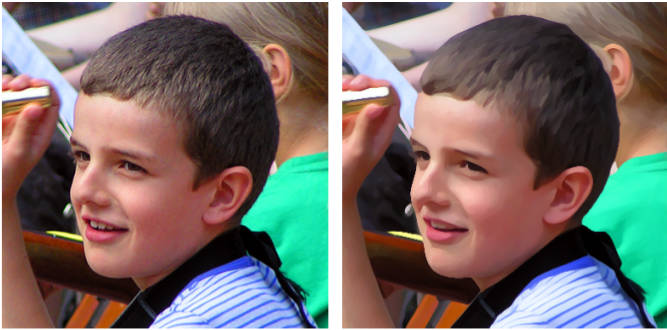
\includegraphics[width=0.7\textwidth]{filterskid}
    \caption{Comparação entre imagem não abstraída (esquerda) e imagem abstraída (direita).}	
    \label{fig:filterskid}
  \end{center}
\end{figure}

Ao nível dos filtros de abstração o estudo será efetuado utilizado o filtro Anisotropic Kuwahara (FAK).

Este filtro consiste numa generalização do filtro Kuwahara que remove alguns artefactos originados na aplicação do filtro original através da adaptação da forma, escala e orientação do filtro à estrutura local das características da imagem \cite{Kyprianidis2009}. Desta forma é produzido um efeito de abstração tipo pintura, onde é removida informação não essencial em zonas de elevado contraste, enquanto são preservados os limites representados nas zonas de menor contraste, tal como demonstrado na figura \ref{fig:filterskid}. As imagens ficam assim com a clareza de uma ilustração, mas preservam a informação direcional tal como nas pinturas a óleo clássicas. Por outro lado, este filtro tira partido da placa gráfica para a realização da abstração das imagens, tornando-se assim particularmente indicado para o processamento de um elevado número de fotografias.

O filtro em questão foi também utilizado anteriormente, e com resultados positivos, em abstração de imagens para a recuperação de informação multimédia. 

Tendo em conta os fatores apresentados consideramos que este filtro é o mais adequado para a utilização no âmbito deste projeto.

\subsection{Coleções de dados}
Ao nível das coleções de dados a analisar serão utilizadas duas coleções de dados Sapo Fama e \textit{Labeled Faces in the Wild}.

\subsubsection{\textit{Labeled Faces in the Wild}}
A coleção \textit{Labeled Faces in the Wild (LFW)} é uma base de dados fotográfica desenhada especificamente para o estudo do problema de reconhecimento facial, particularmente em situações onde as condições de captura das imagens não possuem restrições. Esta coleção possuí 13233 imagens, de 5749 pessoas diferentes, sendo que dessas pessoas 1680 possuem mais do que uma imagem na galeria. O uso desta galeria no âmbito desta dissertação permitirá efetuar uma análise dos resultados obtidos num conjunto de dados standard e já previamente analisado por outros investigadores, assim como agilizar os testes dos sistemas desenvolvidos uma vez que a coleção já se encontra preparada especificamente para o estudo do desempenho de sistemas de reconhecimento facial automático. Nas figuras \ref{fig:galeria}, \ref{fig:gp} e \ref{fig:gn} encontram-se representados alguns exemplos das imagens contidas nesta coleção e respetivas anotações.

\subsubsection{Sapo Fama}
\begin{figure}[h]
  \begin{center}
    \leavevmode
    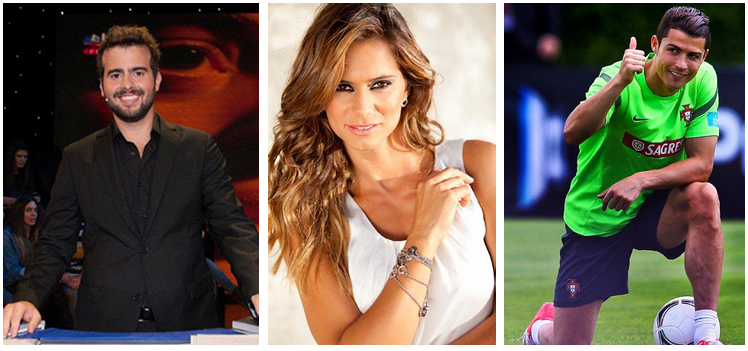
\includegraphics[width=0.9\textwidth]{sapoFama.png}
    \caption{Exemplos de imagens da coleção Sapo Fama.}	
    \label{fig:sapoFama}
  \end{center}
\end{figure}
A coleção Sapo Fama foi disponibilizada no âmbito da integração desta dissertação no laboratório de investigação da Sapo da Universidade do Porto. Esta galeria multimédia agrega uma coleção de imagens utilizadas na plataforma online de notícias sobre personalidades públicas da Sapo, capturadas num grande número de eventos com condições de iluminação, pose e expressão facial muito variáveis. Para além disso, a cada imagem encontra-se ainda associada uma descrição textual. As imagens contidas nesta coleção representam uma oportunidade única de avaliação do sistema desenvolvido numa biblioteca de imagens real e com elevado valor comercial. Na figura \ref{fig:sapoFama} encontram-se representados alguns exemplos das imagens contidas nesta coleção.

Para a utilização deste conjunto de dados será ainda necessário efetuar a preparação do mesmo nomeadamente através da extração e segmentação das diversas entidades presentes em cada imagem, assim como da normalização das imagens em termos de dimensão.

\section{Avaliação Performance}
A avaliação da performance dos sistemas de reconhecimento facial é normalmente efetuada em duas situações específicas: identificação e verificação de faces. No âmbito da avaliação desses sistemas designam-se de $amostras$ $biometricas$ as capturas de características de uma pessoa que permitem efetuar o seu reconhecimento. Dependendo do sistema essas amostras podem ser apenas uma imagem, um conjunto de imagens ou até um vídeo. Designa-se ainda de $prova$ a amostra biométrica apresentada ao sistema para ser reconhecida.

Para uma avaliação precisa dos sistemas automáticos de reconhecimento facial são necessários três conjuntos de imagens:
\begin{figure}[h]
  \begin{center}
    \leavevmode
    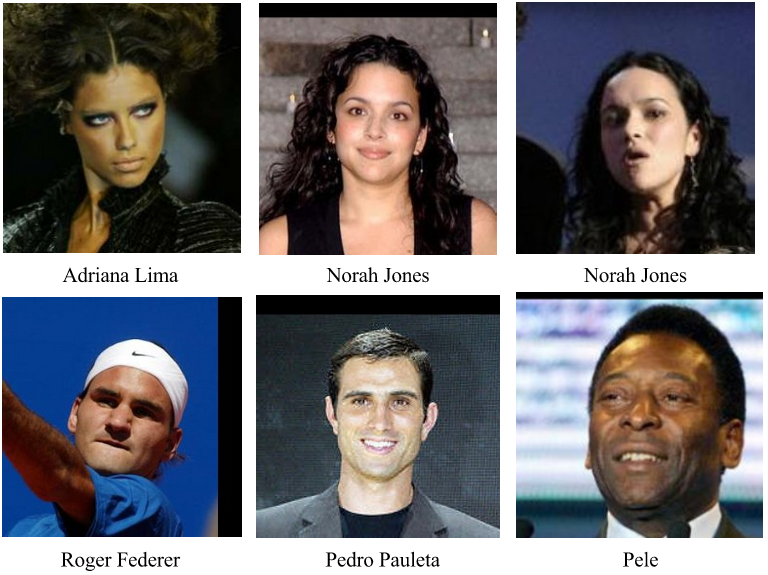
\includegraphics[width=0.9\textwidth]{galeria.png}
    \caption{Galeria com faces conhecidas pelo sistema e respectivas anotações.}	
    \label{fig:galeria}
  \end{center}
\end{figure}
O primeiro, conjunto $\mathscr{G}$, designado de galeria, contem amostras biométricas das pessoas já conhecidas pelo sistema. Um exemplo de imagens da galeria pode ser visto na figura \ref{fig:imggaleria}

\begin{figure}[h]
  \begin{center}
    \leavevmode
    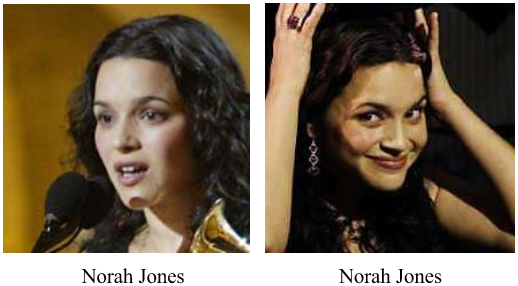
\includegraphics[width=0.6\textwidth]{gp.png}
    \caption{Imagens de pessoas conhecidas pelo sistema, mas não presentes na galeria.}	
    \label{fig:gp}
  \end{center}
\end{figure}
O segundo grupo de imagens é o conjunto $\mathscr{P}_\mathscr{G}$, engloba o conjunto de provas de pessoas conhecidas pelo sistema, mas que são diferentes das amostras biométricas presentes na galeria. Um exemplo de imagens deste conjunto pode ser visto na figura \ref{fig:gp}, onde se encontram representadas imagens da cantora Norah Jones, mas que são diferentes das imagens presentes no conjunto $\mathscr{G}$.

\begin{figure}[h]
  \begin{center}
    \leavevmode
    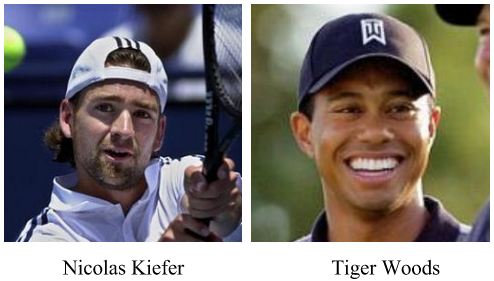
\includegraphics[width=0.6\textwidth]{gn.png}
    \caption{Imagens de pessoas não conhecidas pelo sistema.}	
    \label{fig:gn}
  \end{center}
\end{figure}
O último conjunto é designado de $\mathscr{P}_\mathscr{N}$, e corresponde ao conjunto de provas de pessoas não presentes na galeria. Essas imagens são também muitas vezes designadas de impostores, uma vez que servem para testar as situações em que o sistema identifica erradamente pessoas desconhecidas pelo sistema como pessoas presentes na galeria. Um exemplo deste conjunto de imagens encontra-se representado na figura \ref{fig:gn}

Quando uma prova $p_j$ é apresentada ao sistema, essa prova é então comparada a cada amostra biométrica da galeria $g_i$, resultando dessa comparação o respetivo índice de similaridade (\textit{similarity score}), $s_{ij}$. Este índice é designado de $match$ $score$, caso $g_i$ e $p_j$ sejam amostras da mesma pessoa, caso não o sejam é designado de $nonmatch$ $score$.

A função $id()$ retorna a identidade de uma amostra biométrica, em que $id(p_j) = id(g^*)$, sendo $g^*$ a única correspondência de $p_j$ na galeria e $s_{*j}$ o respetivo índice de similaridade.

De seguida encontra-se descrita brevemente a forma como é efetuada a avaliação da performance dos sistemas de reconhecimento facial para os casos de identificação e verificação.

\subsection{Identificação}
Tal como referido no capítulo \ref{chap:reco} deste relatório, em sistemas de reconhecimento facial automático o problema de identificação consiste na determinação da identidade de uma amostra biométrica (prova) fornecida ao sistema.

Na identificação de uma dada prova são calculados os índices de similaridade para todas as amostras na galeria, e ordenados os seus resultados. Uma prova $p_j$ tem ranking $n$ se o seu índice de similaridade for o enésimo maior índice de similaridade. Caso haja empates nos índices de similaridade é necessário resolver esses empates para determinar o ranking de uma prova, havendo para isso três métodos: otimista, pessimista e média. No método otimista, uma prova é associada ao ranking mais alto possível, obtido pelo número de índices estritamente maiores do que $s_{*j}$ mais um ($|> s_{*j}| + 1$). Na abordagem pessimista, um prova é associada ao ranking mais baixo possível, sendo esse devolvido pelo número de índices maiores ou iguais a $s_{*j}$ mais um ($|\geqslant s_{*j}| + 1$). Na média, tal como o seu nome indica é efetuada uma média entre os valores obtidos pelos métodos pessimista e otimista, sendo esta a abordagem mais utilizada. 

A performance da identificação em sistemas de reconhecimento facial pode ser avaliada em taxa de deteção e identificação e taxa de falso-alarme:

 \begin{description}
 \item[Taxa de deteção e identificação $(T_{DI})$:] Percentagem de provas do conjunto $\mathscr{P}_\mathscr{G}$ que são corretamente  identificadas. Uma prova é corretamente identificada caso o índice de similaridade para o seu $match$ $score$ seja seja maior do que um limite operacional pré-definido $\tau$.
\begin{equation}
 T_{DI}(\tau, n) = \frac{|\{p_j:p_j \in \mathscr{P}_\mathscr{G}, rank(p_j) \leqslant n, s_{*j} \geqslant \tau\}|}{|\mathscr{P}_\mathscr{G}|}
\end{equation}
 Em que no caso de se pretender apenas determinar a identificação da pessoa é devolvido apenas o \textit{top match}, ou seja o resultado com ranking $n=1$. Caso contrário, podem ser devolvidos todos os primeiros $n$ resultados com índice de similaridade superior ao limite operacional estabelecido.
 
  \item[Taxa de falso-alarme $(T_{FA})$:] Percentagem de impostores identificados erradamente, ou seja, percentagem de pessoas do conjunto de provas $\mathscr{P}_\mathscr{N}$, identificadas como alguém presente na galeria $\mathscr{G}$.  
\begin{equation}
 T_{FA}(\tau) = \frac{|\{p_j:p_j \in \mathscr{P}_\mathscr{N}, s_{ij} \geqslant \tau\}|}{|\mathscr{P}_\mathscr{N}|}
\end{equation}
\end{description}

Um sistema de reconhecimento facial ideal teria uma taxa de deteção e identificação de 1.0 e uma taxa de falso-alarme de 0.0.

\subsection{Verificação}
Em situações de verificação da identidade, para além de uma amostra biométrica ($prova$) é também fornecida ao sistema a identidade da pessoa que se pretende identificar. Cabe ao sistema determinar se a identidade e amostra fornecidas pertencem à mesma pessoa. O sistema compara então a prova à amostra biométrica guardada na galeria, da pessoa a quem corresponde a identidade fornecida. Da comparação efetuada resulta o índice de similaridade entre a prova fornecida e os dados já armazenados no sistema.

Em termos formais, a verificação pode ser avaliada pela taxa de verificação e taxa de falso-alarme, as quais podem ser descritas da seguinte forma:

\begin{description}
 \item[Taxa verificação $(T_{V})$:] Percentagem de provas do conjunto $\mathscr{P}_\mathscr{G}$ que são corretamente verificadas. O sistema aceita como verdadeira a identidade fornecida caso o índice de similaridade calculado seja superior a um  limite operacional fornecido.

\begin{equation}
 T_{V}(\tau, n) = \frac{|\{p_j:p_j \in \mathscr{P}_\mathscr{G}, s_{ij} \geqslant \tau, id(g_i)=id(p_j)\}|}{|\mathscr{P}_\mathscr{G}|}
\end{equation}

  \item[Taxa de falsa-aceitação $(T_{FA})$:] Percentagem de impostores aceites erradamente, ou seja, percentagem de pessoas do conjunto de provas $\mathscr{P}_\mathscr{N}$, verificadas como alguém presente na galeria $\mathscr{G}$.
  
\begin{equation}
 T_{FA}(\tau) = \frac{|\{p_j:p_j \in \mathscr{P}_\mathscr{N}, s_{ij} \geqslant \tau\}|}{|\mathscr{P}_\mathscr{N}||\mathscr{G}|}
\end{equation}
\end{description}

\begin{figure}[h]
  \begin{center}
    \leavevmode
    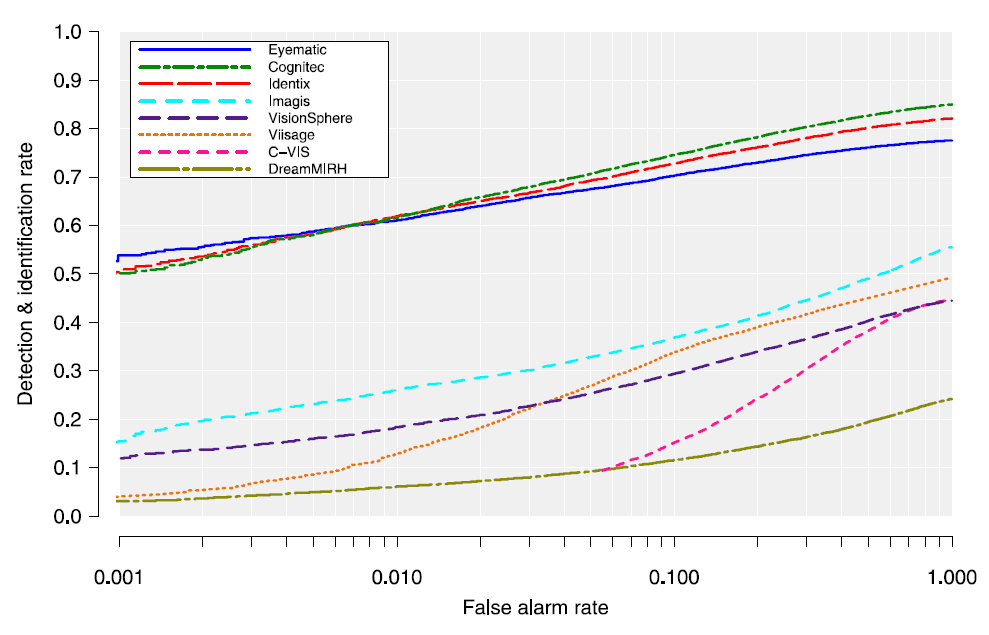
\includegraphics[width=0.8\textwidth]{roc.png}
    \caption{ROC.}	
    \label{fig:roc}
  \end{center}
\end{figure}
A modificação do valor de $\tau$ tem influência direta nas percentagens de deteção e/ou verificação e de falsos-alarmes calculadas. Ao aumentar o limite operacional, ambas as taxas diminuem, não sendo por isso possível maximizar ambos os valores, uma vez que existe sempre um compromisso entre o aumento da taxa de deteção e identificação e o aumento do número de falsos-alarmes. Este compromisso é tradicionalmente representado num gráfico do tipo \textit{receiver operating characteristic} (ROC). Um exemplo de um ROC encontra-se representado na figura \ref{roc}, com um ranking constante de 1. 

\begin{figure}[h]
  \begin{center}
    \leavevmode
    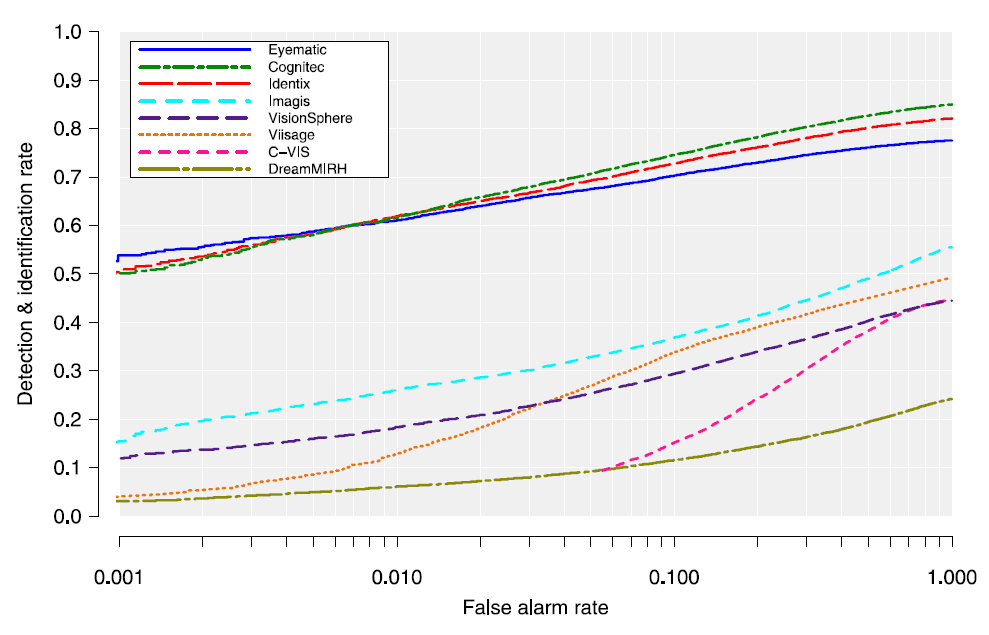
\includegraphics[width=0.8\textwidth]{roc.png}
    \caption{ROC2.}	
    \label{fig:roc2}
  \end{center}
\end{figure}
Outra forma de representar a performance de sistemas de reconhecimento facial é em função do ranking das provas presentes na galeria e encontra-se representada na figura \ref{roc2}. Nesta figura, o eixo vertical representa a taxa de deteção e reconhecimento e o eixo horizontal o ranking numa escala logarítmica. Cada curva representa a performance do mesmo sistema com uma diferente taxa de falso-alarme.

\section{Resultados Esperados}
Tendo em conta os resultados anteriormente observados no recurso à utilização de filtros de abstração para a ilustração automática de texto e o estado da arte da área de reconhecimento facial automático em imagens, esperamos, no contexto desta dissertação, determinar o impacto do uso da abstração de imagens no processo de reconhecimento facial automático, nomeadamente nos seguintes pontos:
\begin{itemize}
\item Eficácia do Reconhecimento;
\item Necessidades de Processamento das imagens;
\item Necessidades de Armazenamento das imagens.
\end{itemize}
Em cada um dos pontos identificados anteriormente pretendemos determinar, qual o impacto ao nível na performance (melhoria ou perda de eficácia) com o uso de abstração de imagens, e qual o compromisso existente entre a eficácia do reconhecimento e as necessidades de processamento e armazenamento das imagens.

\section{Plano de Trabalho}

\begin{figure}[t]
  \begin{center}
    \leavevmode
    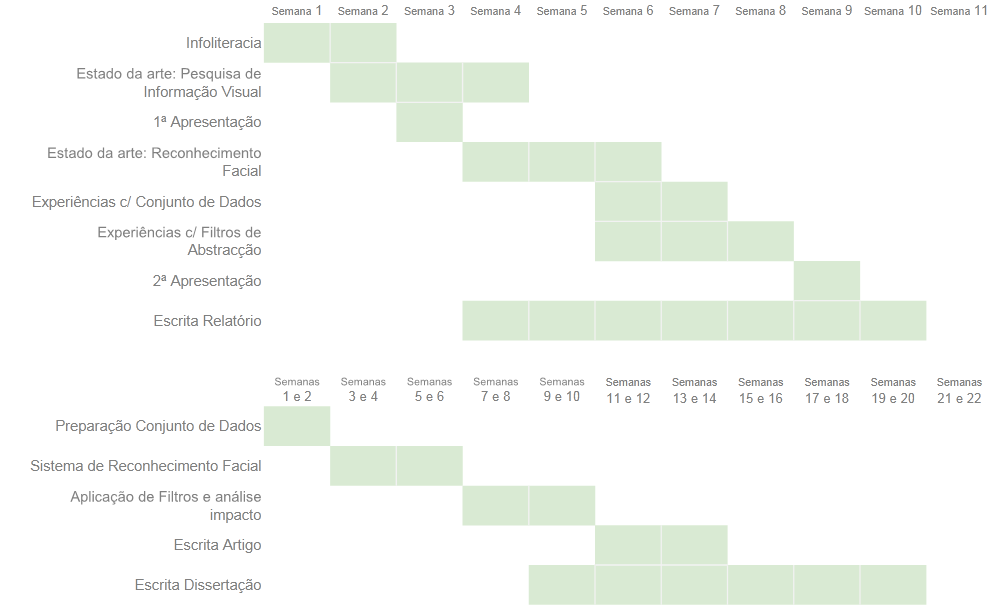
\includegraphics[width=1\textwidth]{GantSemSemanas}
    \caption{Plano de Trabalho 1º e 2º Semestres}	
    \label{fig:planotrabalho}
  \end{center}
\end{figure}

//Novo gant só com 2º semestre?

%Adicionalmente propõe-se também o desenvolvimento de um sistema de reconhecimento facial de personalidades que integre a abstração de imagens no processo de reconhecimento facial. Este sistema deverá ser capaz de detetar as faces presentes numa imagem e apresentar uma lista de possíveis entidades nela contidas.

\chapter{Plano de Trabalho} \label{chap:planotrabalho}

Neste capítulo...

\section{Resumo ou Conclusões}

Aliquam erat volutpat. Nunc pede ipsum, porttitor eu, bibendum non,
bibendum nec, nisl. Maecenas eget mauris. Nullam pulvinar. Curabitur
rutrum commodo est. Nam sapien pede, interdum eu, accumsan ultrices,
venenatis sit amet, tellus. Praesent ac ante bibendum enim varius
suscipit. Donec enim. Proin nisi. Quisque libero turpis, varius ut,
elementum vel, pulvinar sed, nunc. 

\chapter{Conclusões e Perspetivas Futuras} \label{chap:conclusao}

\section{Conclusões}
A investigação realizada no âmbito desta dissertação teve como principal objetivo estudar o impacto do uso da abstração de imagens no processo de reconhecimento facial automático, assim como de um conjunto de tarefas de pré-processamento efetuadas sobre as imagens. Tendo em vista esse objetivo, foi desenvolvido o sistema de reconhecimento facial Visage. Para uma dada imagem fornecida ao sistema Visage, é aplicada sobre ela uma cadeia de pré-processamento, na qual a abstração de imagens se encontra incluída, e é efetuado posteriormente o seu reconhecimento, sendo devolvida uma lista ordenada de possíveis entidades contidas na imagem original.

Através da análise do estado da arte apresentada é possível concluir que o reconhecimento facial em imagens é um tema atual e onde se tem verificado um interesse crescente devido às suas múltiplas áreas de aplicação, assim como ao elevado valor comercial tradicionalmente associado a este tipo de soluções. 

O problema de reconhecimento facial é, no entanto, um problema complexo que integra, também ele, um conjunto de sub-problemas  complexos. Estes sub-problemas, aliados as múltiplas áreas de aplicação do reconhecimento facial, fazem com que exista uma grande variação do desempenho dos sistemas existentes, a qual se encontra diretamente relacionada com as condições de utilização dos mesmos, nomeadamente ao no que diz respeito às galerias de imagens utilizadas. A este nível, em situações onde as condições de captura das imagens são controladas e existe uma cooperação ativa por parte dos utilizadores os resultados obtidos são muito satisfatórios, sendo mesmo considerado que, nestas situações, o problema se encontra praticamente resolvido. Em contraste, em situações de captura não controladas e onde exista uma variação da iluminação, pose e expressão dos indivíduos este é ainda um problema desafiante e onde se verifica necessidade de investigação na atualidade.

Por outro lado, os filtros de abstração são ferramentas computacionalmente eficazes de abstração de informação, sendo tradicionalmente utilizados para comunicar mais eficazmente uma mensagem visual. Para além disso, o uso destes filtros para a pesquisa baseada em conteúdos com vista a ilustração automática de texto demonstrou resultados positivos quer ao nível da informação retornada, quer ao nível das necessidades de armazenamento das imagens.

Tendo em conta a pertinência do estudo no âmbito do reconhecimento facial automático em situações de captura de imagens não controladas, assim como a inexistência de estudos relativos ao impacto da utilização de filtros de abstração no processo de reconhecimento, a investigação levada a cabo no âmbito desta dissertação contribui de forma relevante para o conhecimento existente na área. 

Ao nível das avaliações efetuadas, é possível concluir que a deteção e segmentação correta das faces constituem as etapas de pré-processamento mais relevantes para a obtenção de resultados positivos no reconhecimento dos indivíduos, independentemente do algoritmo de reconhecimento utilizado. Por outro lado, a normalização do contraste das imagens através da equalização do seu histograma revela uma melhoria significativa nos resultados obtidos com particular ênfase no algoritmo \textit{Eigenfaces}. 

Finalmente, a integração da abstração de imagens no processo de reconhecimento apresenta um compromisso entre a diminuição da necessidade de processamento e armazenamento necessárias, com a ligeira diminuição da eficácia do reconhecimento. A este nível destaca-se o filtro Kuwahara anisotrópico, o qual representa o maior grau de abstração dos filtros utilizados, permitindo uma diminuição considerável do tamanho da galeria processada, mas que regista também um maior impacto no desempenho do reconhecimento.

Por último, a implementação do sistema Visage com base em uma biblioteca de código aberto permite também alargar o número de soluções atualmente existentes a este nível, ao mesmo tempo que constitui uma base sólida para o desenvolvimento de futuras aplicações que tirem partido do reconhecimento facial automático em imagens no seu funcionamento.

\section{Perspetivas Futuras}
O sistema de reconhecimento facial desenvolvido, assim como as avaliações efetuadas, vão de encontro aos objetivos traçados no âmbito desta dissertação, permitindo contribuir ativamente para o conhecimento existente acerca da aplicação de filtros de abstração no processo de reconhecimento facial em imagens. De seguida, encontra-se resumido algum do trabalho futuro com vista a melhorar o sistema de reconhecimento facial Visage, assim como expandir as conclusões da avaliação efetuada.

A primeira etapa de pré-processamento aplicada no sistema Visage corresponde à deteção das faces presentes numa imagem. Nesta fase, é apenas considerada a existência de uma cara relevante na imagem e é utilizado um classificador em cascata treinado para caras em posição frontal. A expansão desta etapa de pré-processamento, permitindo a identificação de múltiplas pessoas na mesma imagem, seria um próximo passo na melhoria da etapa de deteção facial. A utilização de vários classificadores diferentes correspondentes às múltiplas poses representadas nas diferentes imagens permitiria também efetuar uma deteção facial mais robusta, para além de possibilitar a criação de modelos de reconhecimento facial focados em reconhecer imagens de uma pessoa com uma pose específica.

Ao nível das restantes tarefas de pré-processamento aplicadas antes de efetuar a abstração das imagens existe também algum espaço para melhoria. Em primeiro lugar, o processo de alinhamento das imagens poderia ser melhorado de forma a o tornar mais robusto e ter em consideração a pose de uma face no seu alinhamento. No que diz respeito às técnicas de normalização do contraste, a diferença obtida com recurso à equalização do histograma e com recurso à técnica \textit{CLAHE} indicam também que esta é uma área onde existe um espaço para melhoria.

A abstração de imagens foi efetuada com recurso a três filtros distintos, os quais representam três graus de abstração de complexidade diferente. No âmbito de trabalho futuro a avaliação de outras técnicas de abstração de imagens poderá ser considerada.

A arquitetura do sistema Visage baseou-se na implementação de múltiplas aplicações do tipo caixa preta, onde para um conjunto de dados de entrada é produzido um resultado específico, sem que para isso seja necessário ter um conhecimento aprofundado acerca do funcionamento do sistema. A integração e eventual adaptação deste sistema a uma arquitetura cliente-servidor poderia permitir uma utilização dos métodos implementados de uma forma mais simples e intuitiva por parte de outras aplicações.


 

%% Comment next 2 commands if numbered appendices are not used
%%\appendix
%%\chapter{Avaliação \textit{Closed-set Identification}} \label{ap1:closed-set}
Nas tabelas abaixo encontram-se representados os resultados obtidos na avaliação \textit{Closed-set Identification}, para as nove galerias avaliadas, agrupados pelo algoritmo utilizado.

\begin{table}[h]
    \begin{center}
    \caption{Média dos resultados obtidos para o algoritmo \textit{Eigenfaces} nos 4 conjuntos de teste avaliados.}	
	\begin{tabular}{c|p{1.2cm}p{1.1cm}p{1.1cm}p{1.7cm}p{1.5cm}p{1.2cm}p{1.2cm}p{1.2cm}p{1.2cm}}
	Rank & Original & Cropped & Masked & Normalized & Equalized & CLAHE & Gaussian & Bilateral & AKF \\ 
	\hline\hline
	1 & 12.9\% & 25.9\% & 28.1\% & 30.0\% & 43.0\% & 40.9\% & 43.4\% & 42.7\% & 41.0\% \\ 
	2 & 18.3\% & 34.3\% & 37.7\% & 39.1\% & 55.3\% & 52.5\% & 55.5\% & 54.1\% & 51.5\% \\ 
	3 & 23.8\% & 40.2\% & 43.4\% & 45.9\% & 60.7\% & 59.8\% & 61.2\% & 60.7\% & 58.9\% \\ 
	4 & 27.9\% & 46.3\% & 47.9\% & 52.1\% & 64.6\% & 64.1\% & 65.3\% & 64.3\% & 62.5\% \\ 
	5 & 31.9\% & 50.0\% & 52.8\% & 56.7\% & 68.3\% & 68.0\% & 68.5\% & 67.9\% & 66.1\% \\ 
	6 & 35.7\% & 53.8\% & 55.7\% & 60.3\% & 70.8\% & 71.4\% & 71.7\% & 70.8\% & 69.5\% \\ 
	7 & 39.4\% & 57.0\% & 58.3\% & 62.9\% & 73.1\% & 73.6\% & 73.5\% & 72.9\% & 72.0\% \\ 
	8 & 41.3\% & 60.1\% & 61.1\% & 65.7\% & 74.6\% & 75.6\% & 75.5\% & 74.8\% & 73.6\% \\ 
	9 & 44.8\% & 62.2\% & 63.9\% & 68.6\% & 76.1\% & 78.0\% & 76.5\% & 76.2\% & 75.4\% \\ 
	10 & 47.6\% & 64.0\% & 65.8\% & 70.4\% & 77.9\% & 80.3\% & 78.3\% & 77.7\% & 76.4\% \\ 
	11 & 49.4\% & 66.1\% & 68.3\% & 72.7\% & 80.1\% & 81.4\% & 79.9\% & 79.0\% & 78.0\% \\ 
	12 & 51.9\% & 68.6\% & 70.2\% & 73.9\% & 81.4\% & 82.6\% & 81.4\% & 80.8\% & 79.7\% \\ 
	13 & 53.8\% & 70.8\% & 71.5\% & 75.5\% & 82.6\% & 84.2\% & 82.3\% & 81.9\% & 80.9\% \\ 
	14 & 55.7\% & 71.8\% & 73.1\% & 76.9\% & 83.6\% & 85.3\% & 84.0\% & 84.0\% & 82.5\% \\ 
	15 & 57.7\% & 72.9\% & 75.0\% & 79.7\% & 84.3\% & 86.8\% & 85.0\% & 85.1\% & 83.4\% \\ 
	16 & 59.8\% & 75.2\% & 77.0\% & 80.8\% & 85.6\% & 87.6\% & 85.9\% & 85.7\% & 84.5\% \\ 
	17 & 60.9\% & 76.9\% & 78.2\% & 81.8\% & 87.3\% & 88.5\% & 86.9\% & 86.9\% & 85.8\% \\ 
	18 & 62.0\% & 78.2\% & 79.3\% & 83.5\% & 88.2\% & 89.0\% & 87.6\% & 87.6\% & 86.8\% \\ 
	19 & 63.2\% & 80.1\% & 80.5\% & 84.0\% & 88.9\% & 89.9\% & 88.9\% & 89.0\% & 87.6\% \\ 
	20 & 65.2\% & 81.3\% & 81.5\% & 85.0\% & 89.3\% & 90.6\% & 89.4\% & 89.7\% & 88.5\% \\ 
	21 & 66.4\% & 81.9\% & 82.2\% & 86.0\% & 89.9\% & 91.0\% & 90.3\% & 90.2\% & 88.9\% \\ 
	22 & 67.4\% & 83.2\% & 83.1\% & 87.0\% & 90.8\% & 92.2\% & 90.8\% & 90.6\% & 89.3\% \\ 
	23 & 69.5\% & 84.4\% & 83.9\% & 87.6\% & 91.2\% & 92.6\% & 91.2\% & 91.1\% & 89.9\% \\ 
	24 & 70.8\% & 85.4\% & 85.1\% & 88.5\% & 91.3\% & 93.2\% & 91.5\% & 91.6\% & 90.6\% \\ 
	25 & 72.0\% & 86.2\% & 86.1\% & 89.4\% & 91.4\% & 93.4\% & 91.7\% & 91.8\% & 91.2\% \\ 
	26 & 73.0\% & 86.8\% & 87.1\% & 89.8\% & 91.8\% & 93.5\% & 92.2\% & 92.2\% & 91.8\% \\ 
	27 & 74.5\% & 87.4\% & 87.8\% & 90.8\% & 92.4\% & 93.6\% & 92.6\% & 92.5\% & 92.6\% \\ 
	28 & 75.9\% & 88.0\% & 88.2\% & 91.4\% & 92.9\% & 94.1\% & 93.0\% & 93.0\% & 92.9\% \\ 
	29 & 77.5\% & 88.9\% & 88.6\% & 91.8\% & 93.5\% & 94.3\% & 93.4\% & 93.6\% & 93.3\% \\ 
	30 & 78.4\% & 89.5\% & 89.3\% & 92.3\% & 94.0\% & 95.0\% & 94.4\% & 94.5\% & 94.3\% \\
	\hline\hline
    \end{tabular}
    \label{tab:media_eigen}
    \end{center}
\end{table}	

\begin{table}[h]
    \begin{center}
    \caption{Média dos resultados obtidos para o algoritmo \textit{Fisherfaces} nos 4 conjuntos de teste avaliados.}	
	\begin{tabular}{c|p{1.2cm}p{1.1cm}p{1.1cm}p{1.7cm}p{1.5cm}p{1.2cm}p{1.2cm}p{1.2cm}p{1.2cm}}
	Rank & Original & Cropped & Masked & Normalized & Equalized & CLAHE & Gaussian & Bilateral & AKF \\ 
	\hline\hline
	1 & 30.1\% & 44.2\% & 43.6\% & 42.2\% & 47.3\% & 45.8\% & 44.4\% & 44.2\% & 42.7\% \\ 
	2 & 41.2\% & 53.5\% & 51.7\% & 52.9\% & 55.5\% & 54.3\% & 52.4\% & 52.8\% & 52.2\% \\ 
	3 & 49.2\% & 59.1\% & 59.5\% & 60.0\% & 60.4\% & 60.8\% & 58.3\% & 60.0\% & 58.8\% \\ 
	4 & 55.2\% & 63.6\% & 64.1\% & 64.1\% & 63.9\% & 64.2\% & 62.1\% & 64.5\% & 62.7\% \\ 
	5 & 58.8\% & 66.3\% & 66.5\% & 67.5\% & 67.5\% & 66.8\% & 64.8\% & 67.4\% & 66.4\% \\ 
	6 & 61.4\% & 69.0\% & 68.8\% & 69.1\% & 70.2\% & 70.0\% & 67.6\% & 69.2\% & 71.0\% \\ 
	7 & 64.6\% & 72.0\% & 71.3\% & 70.3\% & 72.6\% & 72.0\% & 69.7\% & 71.7\% & 72.6\% \\ 
	8 & 67.1\% & 73.5\% & 72.5\% & 72.0\% & 74.3\% & 74.8\% & 72.5\% & 73.8\% & 74.6\% \\ 
	9 & 69.0\% & 74.8\% & 73.6\% & 73.7\% & 75.6\% & 76.2\% & 74.3\% & 75.1\% & 76.2\% \\ 
	10 & 71.3\% & 76.6\% & 75.3\% & 75.1\% & 77.5\% & 77.7\% & 75.6\% & 76.8\% & 77.9\% \\ 
	11 & 72.9\% & 77.9\% & 76.7\% & 76.3\% & 79.3\% & 78.2\% & 76.7\% & 78.2\% & 79.1\% \\ 
	12 & 75.6\% & 78.9\% & 77.7\% & 77.5\% & 80.8\% & 79.7\% & 77.8\% & 78.7\% & 80.1\% \\ 
	13 & 77.0\% & 80.0\% & 79.3\% & 79.1\% & 81.7\% & 80.5\% & 79.2\% & 79.7\% & 81.1\% \\ 
	14 & 78.9\% & 81.1\% & 80.2\% & 80.5\% & 82.8\% & 82.1\% & 80.4\% & 80.5\% & 82.4\% \\ 
	15 & 80.6\% & 81.7\% & 81.0\% & 81.1\% & 83.7\% & 83.3\% & 81.7\% & 81.1\% & 83.7\% \\ 
	16 & 82.3\% & 82.9\% & 82.0\% & 82.0\% & 84.3\% & 84.1\% & 82.0\% & 82.6\% & 85.3\% \\ 
	17 & 83.4\% & 83.8\% & 82.7\% & 82.4\% & 85.0\% & 85.4\% & 82.6\% & 83.6\% & 85.5\% \\ 
	18 & 84.2\% & 84.4\% & 83.5\% & 83.1\% & 85.6\% & 86.7\% & 83.3\% & 84.4\% & 86.0\% \\ 
	19 & 85.3\% & 85.6\% & 84.0\% & 84.0\% & 86.4\% & 87.2\% & 84.3\% & 85.3\% & 86.6\% \\ 
	20 & 86.4\% & 86.4\% & 84.4\% & 85.3\% & 87.1\% & 87.7\% & 85.0\% & 86.0\% & 86.9\% \\ 
	21 & 87.6\% & 87.0\% & 85.4\% & 85.8\% & 87.7\% & 87.8\% & 85.8\% & 86.6\% & 88.6\% \\ 
	22 & 88.5\% & 87.6\% & 86.1\% & 86.2\% & 88.1\% & 88.2\% & 86.2\% & 87.1\% & 89.5\% \\ 
	23 & 89.1\% & 88.8\% & 87.0\% & 87.1\% & 88.8\% & 89.0\% & 87.3\% & 88.1\% & 90.4\% \\ 
	24 & 89.5\% & 89.5\% & 87.9\% & 88.0\% & 89.0\% & 89.3\% & 88.1\% & 88.7\% & 90.8\% \\ 
	25 & 90.2\% & 90.2\% & 88.6\% & 88.5\% & 89.1\% & 89.7\% & 88.7\% & 89.0\% & 91.4\% \\ 
	26 & 90.7\% & 90.8\% & 89.1\% & 89.4\% & 89.8\% & 89.8\% & 89.3\% & 89.3\% & 92.0\% \\ 
	27 & 91.2\% & 91.4\% & 89.4\% & 89.9\% & 90.5\% & 90.0\% & 89.6\% & 90.5\% & 92.3\% \\ 
	28 & 91.5\% & 91.8\% & 90.0\% & 90.4\% & 90.7\% & 90.9\% & 90.5\% & 90.9\% & 93.5\% \\ 
	29 & 91.8\% & 92.0\% & 90.5\% & 90.8\% & 91.0\% & 91.2\% & 91.2\% & 91.1\% & 93.8\% \\ 
	30 & 92.2\% & 92.5\% & 91.0\% & 91.3\% & 91.1\% & 91.5\% & 91.5\% & 91.3\% & 94.2\% \\
	\hline\hline
    \end{tabular}
    \label{tab:media_fisher}
    \end{center}
\end{table}

\begin{table}[h]
    \begin{center}
    \caption{Média dos resultados obtidos para o algoritmo \textit{LBPH} nos 4 conjuntos de teste avaliados.}	
	\begin{tabular}{c|p{1.2cm}p{1.1cm}p{1.1cm}p{1.7cm}p{1.5cm}p{1.2cm}p{1.2cm}p{1.2cm}p{1.2cm}}
	Rank & Original & Cropped & Masked & Normalized & Equalized & CLAHE & Gaussian & Bilateral & AKF\\ 
	\hline\hline
	1 & 7.6\% & 47.3\% & 46.8\% & 45.7\% & 49.1\% & 46.1\% & 47.5\% & 42.3\% & 31.5\% \\ 
	2 & 12.5\% & 57.8\% & 57.6\% & 55.9\% & 59.5\% & 54.8\% & 58.3\% & 53.4\% & 41.5\% \\ 
	3 & 15.4\% & 63.1\% & 65.3\% & 63.1\% & 65.0\% & 60.1\% & 61.8\% & 58.8\% & 46.2\% \\ 
	4 & 18.4\% & 67.4\% & 68.8\% & 67.4\% & 68.9\% & 64.5\% & 65.9\% & 63.5\% & 51.7\% \\ 
	5 & 21.6\% & 70.8\% & 71.9\% & 70.6\% & 71.8\% & 68.3\% & 69.4\% & 66.3\% & 56.6\% \\ 
	6 & 23.9\% & 72.8\% & 74.2\% & 72.8\% & 74.1\% & 70.8\% & 72.7\% & 70.2\% & 59.3\% \\ 
	7 & 26.7\% & 74.3\% & 76.0\% & 76.0\% & 75.9\% & 74.3\% & 75.4\% & 72.6\% & 61.6\% \\ 
	8 & 29.8\% & 76.5\% & 77.5\% & 77.5\% & 77.9\% & 76.4\% & 76.8\% & 74.5\% & 62.8\% \\ 
	9 & 32.0\% & 78.5\% & 78.5\% & 79.6\% & 79.2\% & 77.9\% & 78.6\% & 76.4\% & 64.3\% \\ 
	10 & 34.1\% & 79.8\% & 79.9\% & 80.9\% & 80.3\% & 79.5\% & 80.0\% & 78.4\% & 67.3\% \\ 
	11 & 36.0\% & 81.1\% & 81.7\% & 82.7\% & 81.6\% & 81.4\% & 81.5\% & 79.8\% & 69.1\% \\ 
	12 & 37.9\% & 82.4\% & 82.7\% & 83.9\% & 82.1\% & 82.4\% & 82.5\% & 80.5\% & 69.9\% \\ 
	13 & 40.2\% & 83.4\% & 84.0\% & 85.5\% & 83.6\% & 84.0\% & 83.9\% & 81.4\% & 71.5\% \\ 
	14 & 42.0\% & 85.4\% & 85.0\% & 86.4\% & 84.6\% & 85.5\% & 85.7\% & 82.2\% & 72.5\% \\ 
	15 & 43.9\% & 87.1\% & 85.8\% & 87.3\% & 85.6\% & 86.4\% & 86.3\% & 83.3\% & 74.1\% \\ 
	16 & 45.7\% & 88.0\% & 87.1\% & 88.2\% & 86.7\% & 87.3\% & 87.2\% & 84.2\% & 75.0\% \\ 
	17 & 48.1\% & 88.9\% & 88.6\% & 89.2\% & 87.1\% & 88.7\% & 87.8\% & 84.5\% & 76.7\% \\ 
	18 & 50.1\% & 89.6\% & 89.4\% & 89.7\% & 87.8\% & 89.1\% & 89.0\% & 85.3\% & 77.9\% \\ 
	19 & 52.4\% & 89.9\% & 89.7\% & 90.5\% & 88.2\% & 89.9\% & 89.8\% & 85.9\% & 80.0\% \\ 
	20 & 53.8\% & 90.4\% & 90.2\% & 91.0\% & 89.3\% & 90.8\% & 90.7\% & 86.6\% & 81.4\% \\ 
	21 & 56.7\% & 91.1\% & 91.0\% & 91.4\% & 90.0\% & 91.6\% & 91.1\% & 87.0\% & 81.9\% \\ 
	22 & 58.3\% & 91.4\% & 91.1\% & 92.3\% & 90.6\% & 92.4\% & 92.1\% & 87.5\% & 82.5\% \\ 
	23 & 60.1\% & 91.6\% & 91.5\% & 92.8\% & 91.4\% & 92.7\% & 92.2\% & 87.9\% & 83.5\% \\ 
	24 & 62.0\% & 92.1\% & 92.4\% & 93.5\% & 92.0\% & 93.0\% & 92.8\% & 88.4\% & 84.2\% \\ 
	25 & 63.5\% & 92.4\% & 93.0\% & 94.0\% & 92.4\% & 93.3\% & 93.3\% & 89.0\% & 85.0\% \\ 
	26 & 65.4\% & 93.4\% & 93.9\% & 94.3\% & 92.8\% & 93.9\% & 93.9\% & 89.4\% & 85.5\% \\ 
	27 & 67.2\% & 93.6\% & 94.3\% & 94.5\% & 93.1\% & 94.2\% & 94.3\% & 90.2\% & 85.9\% \\ 
	28 & 68.2\% & 94.6\% & 94.5\% & 95.0\% & 93.4\% & 94.6\% & 94.7\% & 90.9\% & 86.6\% \\ 
	29 & 69.2\% & 95.0\% & 94.6\% & 95.4\% & 93.6\% & 95.2\% & 95.0\% & 91.6\% & 87.2\% \\ 
	30 & 70.2\% & 95.4\% & 94.9\% & 95.7\% & 94.2\% & 95.6\% & 95.7\% & 92.1\% & 87.9\% \\
	\hline\hline
    \end{tabular}
    \label{tab:media_lbph}
    \end{center}
\end{table}	

%%----------------------------------------
%% Final materials
%%----------------------------------------

%% Bibliography
%% Comment the next command if BibTeX file not used, 
%% Assumes that bibliography is in ``myrefs.bib''
\PrintBib{myrefs}

%% Index
%% Uncomment next command if index is required, 
%% don't forget to run ``makeindex tese'' command
%\PrintIndex

\end{document}
